%%%%%%%%%%%%%%%%%%%%%%%%%%%%%%%%%%%%%%%%%%%%%%%%%%%%%%%%%%%%%%%%%%%%%%%%%%%%%%%%
%2345678901234567890123456789012345678901234567890123456789012345678901234567890
%        1         2         3         4         5         6         7         8
\documentclass[letterpaper, 10 pt, conference]{ieeeconf}  % Comment this line out
                                                          % if you need a4paper
%\documentclass[a4paper, 10pt, conference]{ieeeconf}      % Use this line for a4

\usepackage{float}
                                                          % paper
% uso paquete bookmark para tener bien los outlines.
\usepackage{bookmark}

% Configuro el idioma.
\usepackage[utf8]{inputenc} % Importante para mantener acentos.
\usepackage[spanish, activeacute]{babel} % Requiere: texlive-lang-spanish. Por primera vez hay que ejecutar: texconfig init> log

% Paquete para poder usar acentos en $$.
\usepackage{mathtools}
%\setmathfont{XITS math}

% Para los diagramas de flujo
\usepackage{tikz}
\usetikzlibrary{shapes.geometric, arrows}

% Elementos del diagrama
\tikzstyle{startstop} = [rectangle, rounded corners, 
minimum width=6em, 
minimum height=2em,
text centered, 
draw=black, 
fill=red!30]

\tikzstyle{io} = [trapezium, 
trapezium stretches=true, % A later addition
trapezium left angle=70, 
trapezium right angle=110, 
minimum width=6em, 
minimum height=2em, text centered, 
draw=black, fill=blue!30]

\tikzstyle{block} = [rectangle, 
minimum width=8em, 
minimum height=3em, 
text centered, 
text width=7.5em, 
draw=black, 
fill=white!30]

\tikzstyle{def} = [rectangle, 
minimum width=14em, 
minimum height=3em, 
text centered, 
text width=12em, 
draw=black, 
fill=purple!30]

\tikzstyle{swap_proccess} = [rectangle, 
minimum width=8em, 
minimum height=2em, 
text centered, 
text width=8em, 
draw=black, 
fill=orange!30]

\tikzstyle{process} = [rectangle, 
minimum width=6em, 
minimum height=2em, 
text centered, 
text width=6em, 
draw=black, 
fill=orange!30]

\tikzstyle{decision} = [diamond, 
minimum width=6em, 
minimum height=6em, 
text centered, 
draw=black, 
fill=green!30]
\tikzstyle{arrow} = [thick,->,>=stealth]

\usepackage{siunitx}

% package to get \url
\usepackage{hyperref}
\hypersetup{
  colorlinks=true,
  linkcolor=magenta,
  filecolor=magenta,
  citecolor=magenta,      
  urlcolor=magenta,
}

% Graficos electrónicos
\usepackage[RPvoltages]{circuitikz}

\IEEEoverridecommandlockouts                              % This command is only
                                                          % needed if you want to
                                                          % use the \thanks command
\overrideIEEEmargins
% See the \addtolength command later in the file to balance the column lengths
% on the last page of the document

\usepackage{graphicx}
\usepackage{graphics}

% styling for matlab/octave code.
\usepackage{matlab-prettifier}
% Configuracion, con esto puede agregar ñ.
\lstset{
  literate={ñ}{{\~n}}1
}

\usepackage{listings}

% The following packages can be found on http:\\www.ctan.org
%\usepackage{graphics} % for pdf, bitmapped graphics files
%\usepackage{epsfig} % for postscript graphics files
%\usepackage{mathptmx} % assumes new font selection scheme installed
%\usepackage{times} % assumes new font selection scheme installed
\usepackage{amsmath} % assumes amsmath package installed
%\usepackage{amssymb}  % assumes amsmath package installed

\title{\LARGE \bf Trabajo Práctico N° 1 Ejercicio 3}

\author{
  Tom\'as Vidal\\
  {\it Control de sistemas biológicos}\\
  {\it Facultad de Ingenier\'ia, UNLP, La Plata, Argentina.}\\
  {\it 17 de Junio, 2025.}
}                                            % <-this % stops a space
% comienzo
% INTRO

% Figura
\newcommand{\image}[2] {
  \begin{figure}[H]
    \centering
    \includegraphics[width=0.43\textwidth]{./#1.png}
    \caption{#2}
    \label{fig:#1}
  \end{figure}
}

% Codigo
% \begin{lstlisting}[style=Matlab-editor]
% % el código va aca
% dispc("HELLO WORLD");
% \end{lstlisting}

\begin{document}
% - - - - - - - - - - - - - - - - - - - - - - - - - - - - - -  TITLE
\begin{titlepage}
	\centering
	\null\vspace{4cm} % Adjust this value to push everything down
	{\LARGE \textbf{Trabajo Práctico N° 3} \par}
	\vspace{2cm}
	{\large Tomás Vidal \par}
	{\itshape Control de sistemas biológicos \par}
	{\itshape Facultad de Ingeniería, UNLP, La Plata, Argentina. \par}
	{\itshape 17 de Junio, 2025. \par}
	\vspace{2cm}
	
\includegraphics[width=0.55\textwidth]{unlp_logo.png}
	\vfill % Pushes the content to properly center vertically
\end{titlepage}
% - - - - - - - - - - - - - - - - - - - - - - - - - - - - - -

\section{Introducción}

Este informe analiza diferentes estrategias de control aplicadas a un sistema biológico, con el objetivo de regular la tasa de crecimiento microbiano ($\mu(s)$) y la concentración de sustrato ($s$). Se comparan métodos como el control proporcional-integral (PI), linealizante y adaptivo, evaluando su desempeño, robustez y adaptabilidad frente a perturbaciones e incertidumbres en los parámetros del modelo. Las simulaciones, realizadas en Simulink, permiten validar teóricamente cada enfoque y ofrecer recomendaciones prácticas para su implementación en biorreactores.

\section{Modelo}
El modelo a simular es el siguiente:

\begin{equation*}
	\begin{cases}
    k_{S1} S + k_N N \xrightarrow{r_x} X + k_{P1} P \\
    k_{S2} S \xrightarrow{r_p} P
	\end{cases}
\end{equation*}

Que se puede llevar al siguiente sistema de ecuaciones:

\begin{equation*}
	\begin{cases}
    \dot{x} = r_{x} \\
    \dot{s} = -K_{s1}r_{x}  + D_{s}(s_{in}  - s) \\
    \dot{s} = -K_{s2}r_{p}  + D_{s}(s_{in}  - s) \\
    \dot{n} = -K_{N}r_{x}  + D_{n}(n_{in}  - n) \\
    \dot{p} = K_{p1}r_{p} \\
	\end{cases}
\end{equation*}

Y representándolo en su forma vectorial se tiene:

\begin{equation}
\begin{bmatrix} \dot{x} \\ \dot{s} \\ \dot{n} \\ \dot{p} \end{bmatrix}
=
\begin{bmatrix} 1 & 0 \\ -K_{s1} & -K_{s2} \\ -K_{N} & 0 \\ K_{P1} & 1 \end{bmatrix}
.
\begin{bmatrix} r_{x} \\ r_{p} \end{bmatrix}
+
\begin{bmatrix} -x \\ s_{in}-s \\ n_{in}-n \\ -p \end{bmatrix}
.
D
\end{equation}

Y si se considera que el nitrógeno se encuentra en saturación, y que en la etapa de producción de biomasa no hay producción de plástico, se puede reducir al siguiente modelo, el cual se emplea en el diseño de los controladores para el resto del informe (\textit{excepto al final que se habla del modelo completo}):

\vspace{0.35cm}

\begin{equation}
\begin{bmatrix} \dot{x} \\ \dot{s} \end{bmatrix}
=
\begin{bmatrix} 1 \\ -K_{s1} \end{bmatrix}
.
r_{x}
+
\begin{bmatrix} -x \\ s_{in}-s \end{bmatrix}
.
D
\end{equation}

\vspace{0.35cm}

Los modelos cinéticos empleados son:

\begin{equation*}
\mu(s,n) = \mu_{\text{max}} \frac{s}{K_S + s + \frac{s^2}{K_{is}}} \cdot \frac{n}{K_n + n}
\end{equation*}

\begin{equation*}
q_p(s,n) = q_{p\text{max}} \frac{s}{K_{ps} + s + \frac{s^2}{K_{ips}}} \cdot \frac{K_{ipn}}{K_{ipn} + n}
\end{equation*}

Que si se considera el caso reducido, donde el nitrógeno está en saturación y no hay producción de plástico, se tiene:

\begin{equation*}
\mu(s) = \mu_{\text{max}} \frac{s}{K_S + s + \frac{s^2}{K_{is}}} 
\end{equation*}

Para realizar la simulación se hizo uso de simulink, a continuación se muestran los dos casos para cuando no se alimenta o se alimenta constantemente con sustrato, y el caso para cuando se alimenta exponencialmente con sustrato.

\begin{figure}[H]
  \centering
  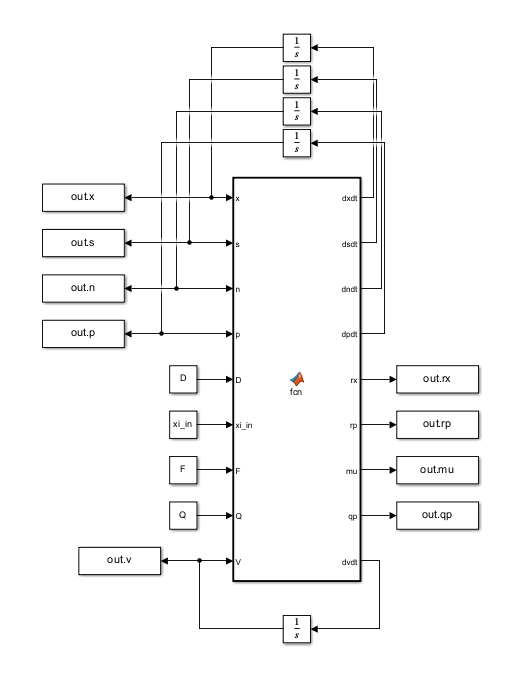
\includegraphics[width=0.43\textwidth]{./Images_tp1/simulink1.png}
  \caption{Simulación para el caso de alimentación constante}
  \label{fig:simulink1}
\end{figure}
\begin{figure}[H]
  \centering
  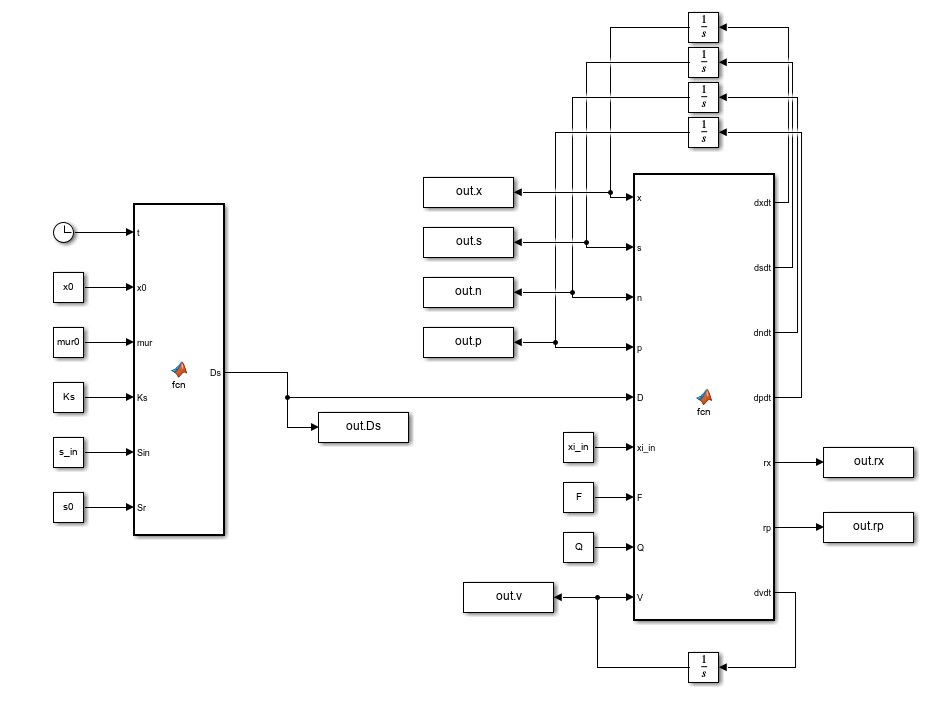
\includegraphics[width=0.43\textwidth]{./Images_tp1/simulink2.png}
  \caption{Simulación para el caso de alimentación exponencial}
  \label{fig:simulink2}
\end{figure}

Para realizar las simulaciones de los diferentes controladores y casos particulares, se hacen variaciones en el simulink, por lo que varían ligeramente de los casos presentados en previamente, pero en esencia sigue siendo el mismo modelo, prácticamente solo se cambia la acción de control.

\section{Sistema sin control}  
Se simula el sistema sin ningún control a forma de referencia.

\begin{figure}[H]
  \centering
  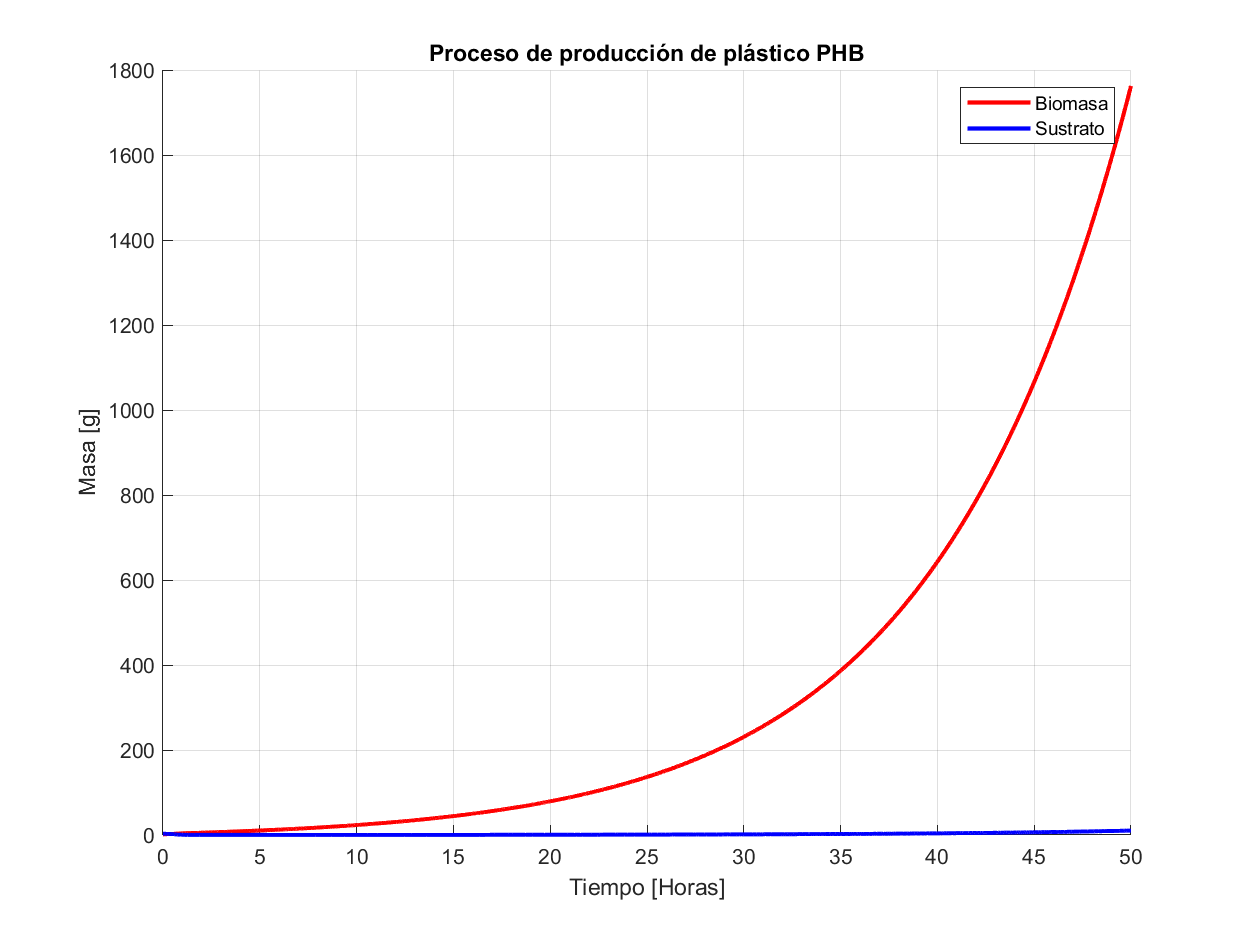
\includegraphics[width=0.43\textwidth]{./Images_tp3/sin_control.png}
  \caption{Sistema sin control}
\end{figure}
\begin{figure}[H]
  \centering
  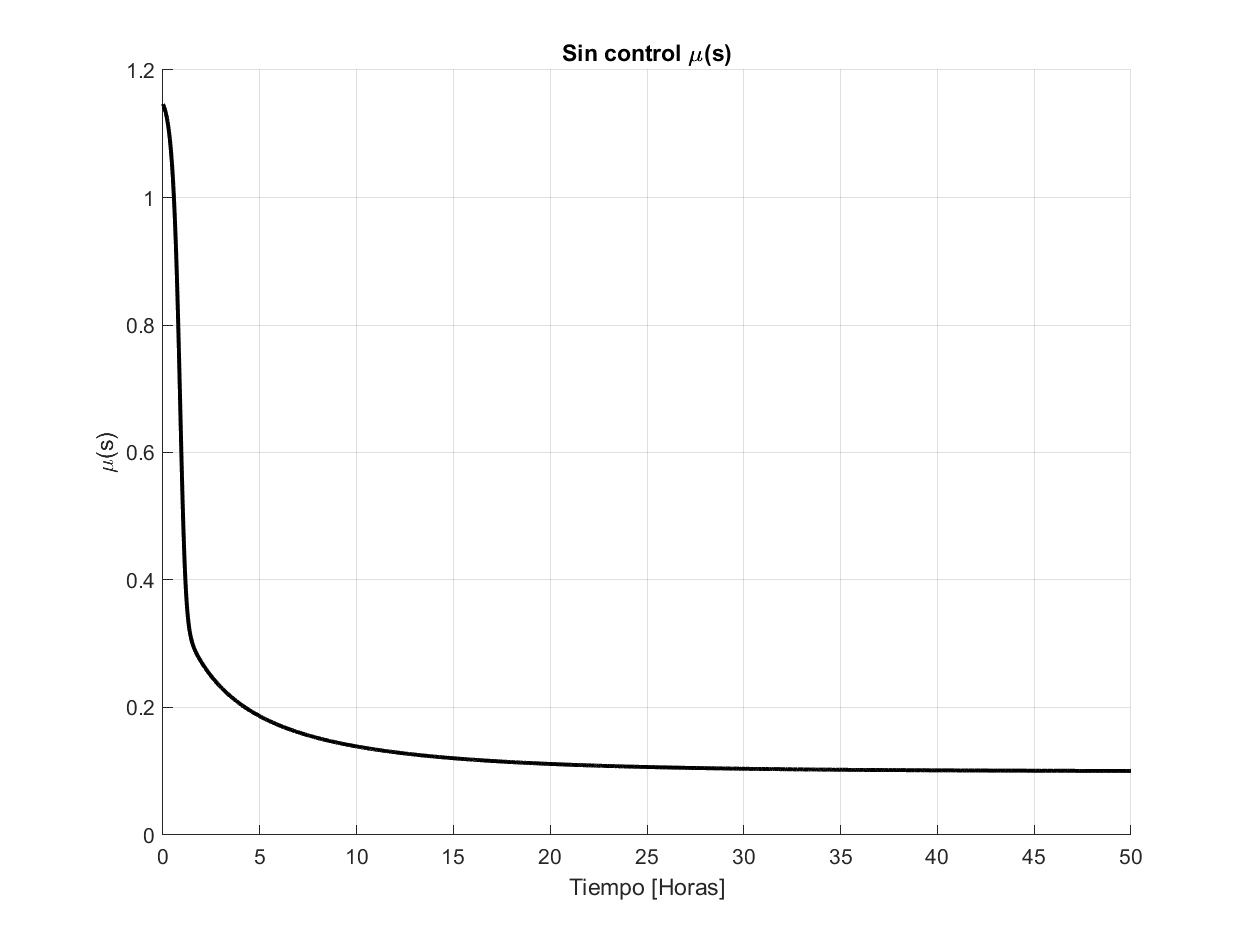
\includegraphics[width=0.43\textwidth]{./Images_tp3/sin_control_mu.png}
  \caption{Sistema sin control (mu)}
\end{figure}

Como se puede ver la biomasa tiene un comportamiento exponencial con respecto al tiempo, y el $\mu(s)$ se establece a un valor, que no es el deseado, por lo que se diseña un controlador para corregirlo.

\section{Control exponencial}
Se implementa un controlador que regula \(\mu(s)\) mediante una alimentación exponencial de sustrato, la acción de control es la dilución:

\begin{equation*}
  u(t) = D = \frac{\lambda X_0 e^{mu_{r}t}}{V}
\end{equation*}

\begin{equation}
D = \frac{\mu_r X_0 k_{s1} e^{\mu_r t}}{(s_{\text{in}} - s_r) V}
\end{equation}

\begin{figure}[H]
  \centering
  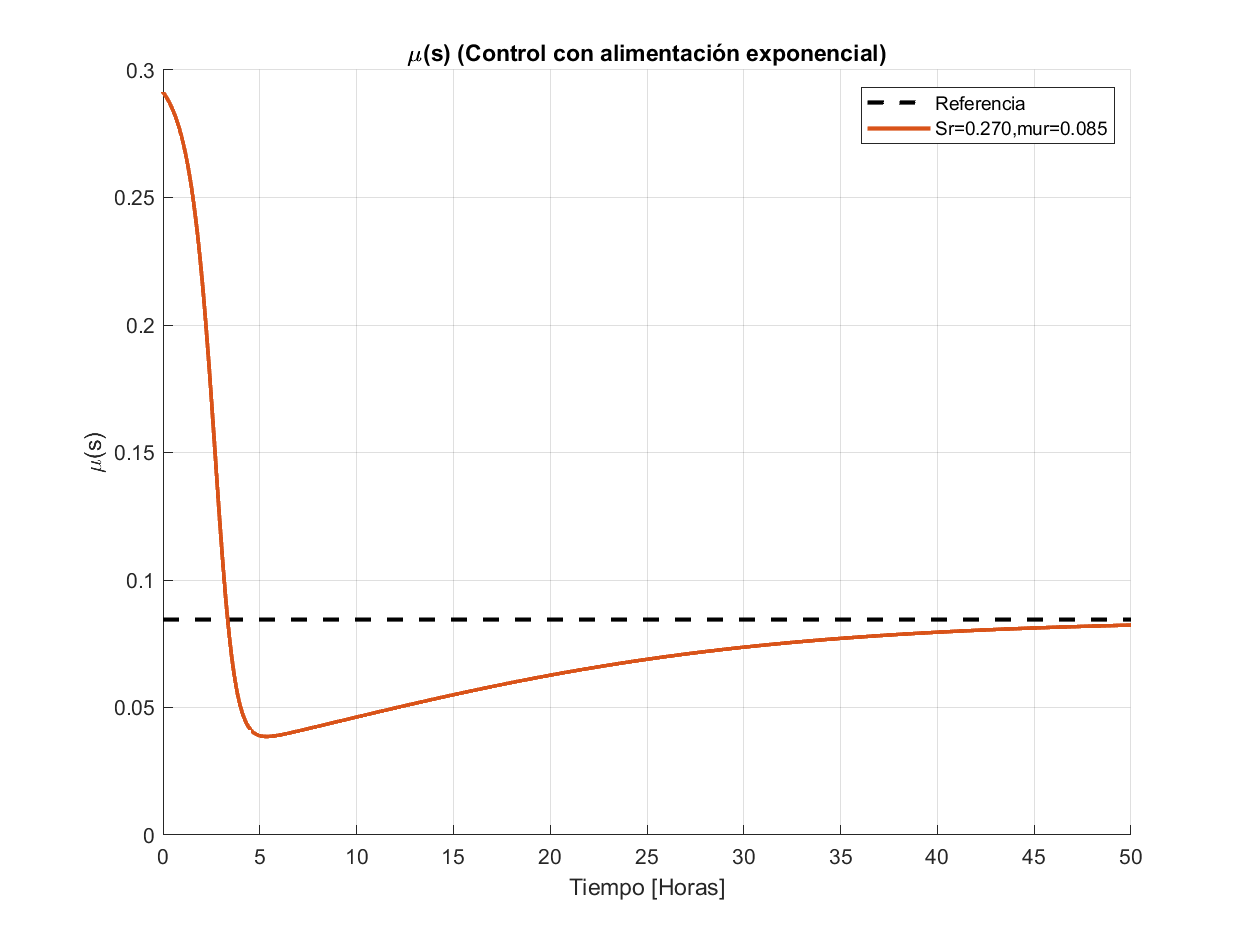
\includegraphics[width=0.43\textwidth]{./Images_tp3/exp.png}
  \caption{Control con alimentación exponencial}
\end{figure}
\begin{figure}[H]
  \centering
  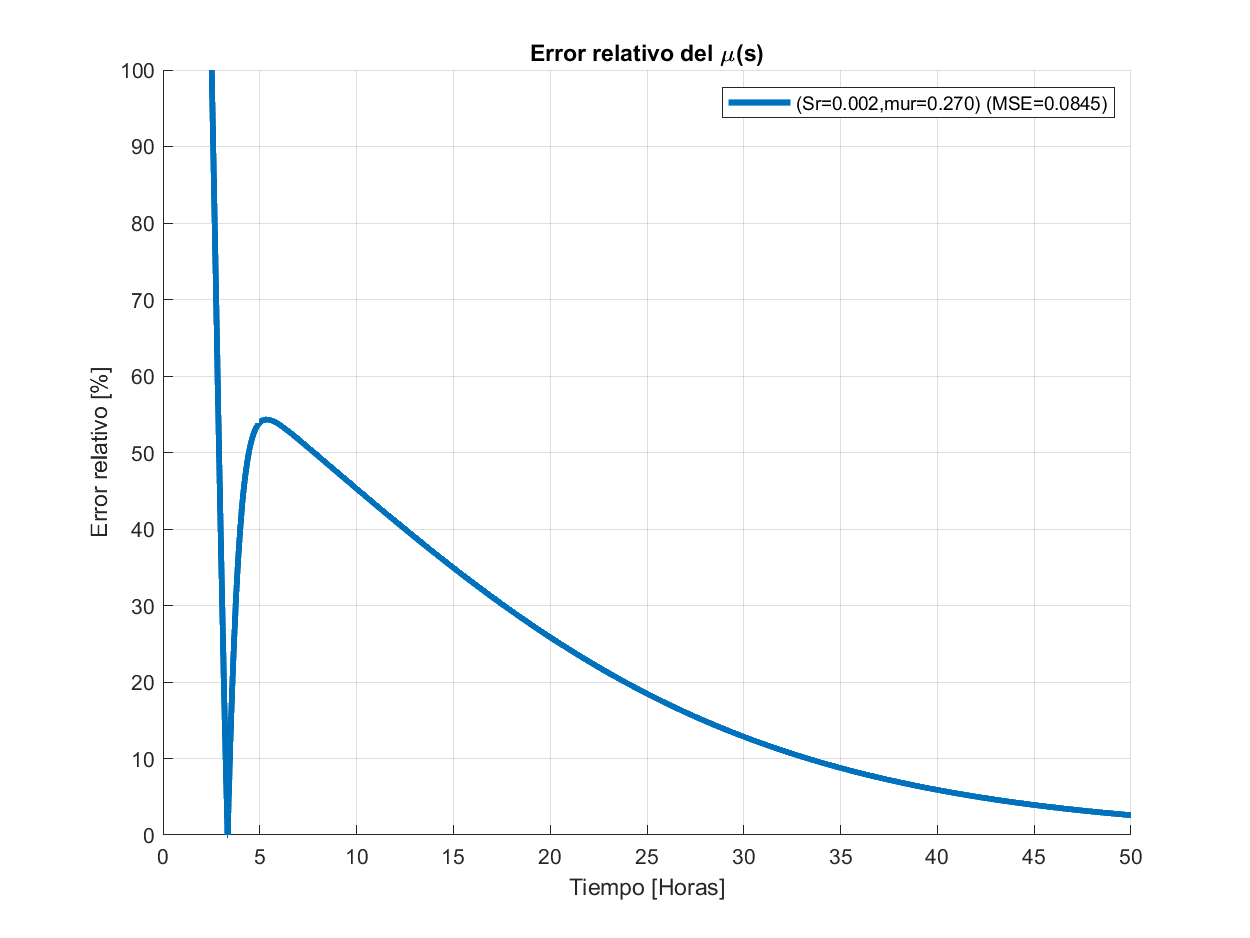
\includegraphics[width=0.43\textwidth]{./Images_tp3/exp_err.png}
  \caption{Error control con alimentación exponencial}
\end{figure}
\begin{figure}[H]
  \centering
  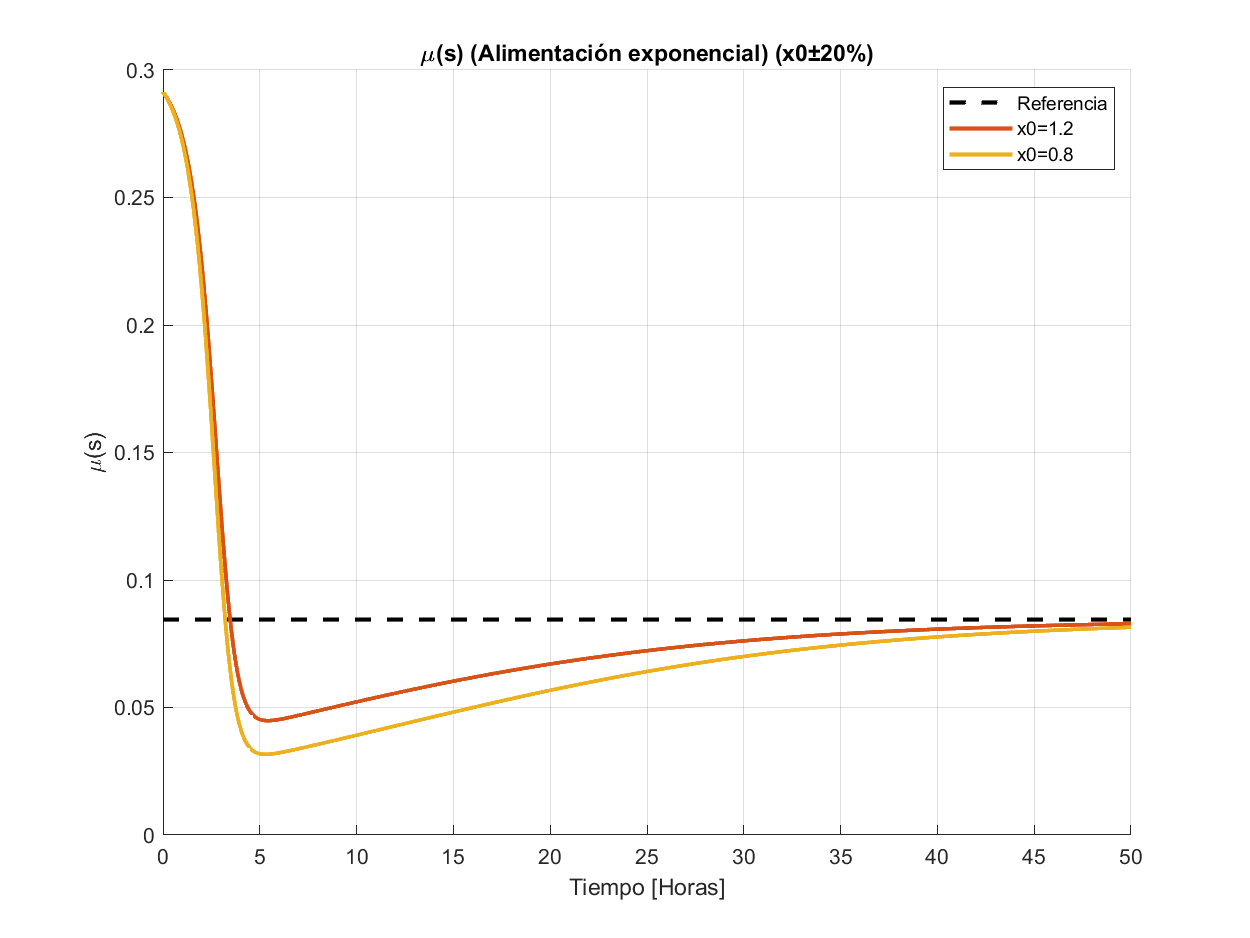
\includegraphics[width=0.43\textwidth]{./Images_tp3/exp_x0.png}
  \caption{Control con alimentación exponencial (se varía $x_{0}$)}
\end{figure}
\begin{figure}[H]
  \centering
  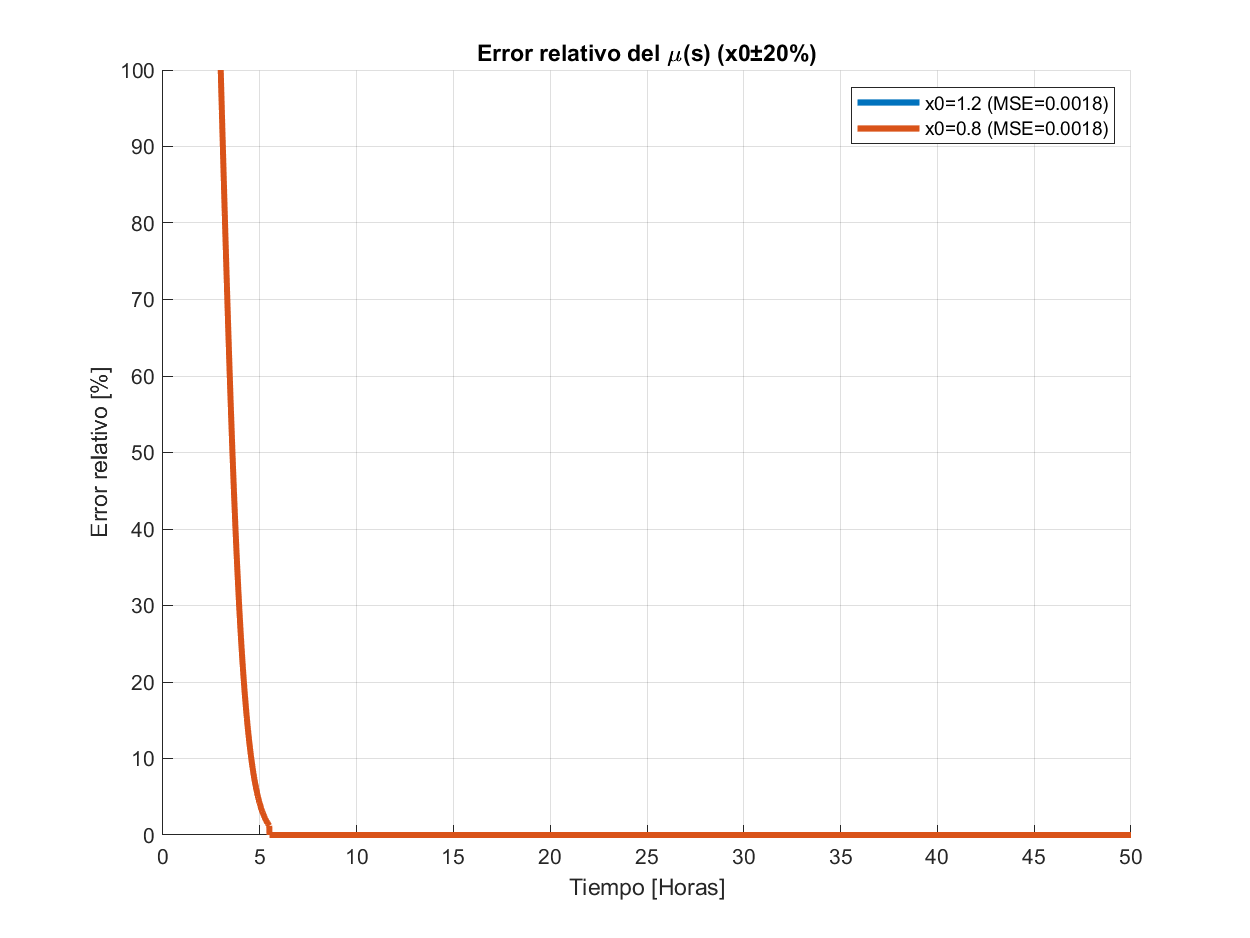
\includegraphics[width=0.43\textwidth]{./Images_tp3/exp_err_x0.png}
  \caption{Error control con alimentación exponencial (se varía $x_{0}$)}
\end{figure}
\begin{figure}[H]
  \centering
  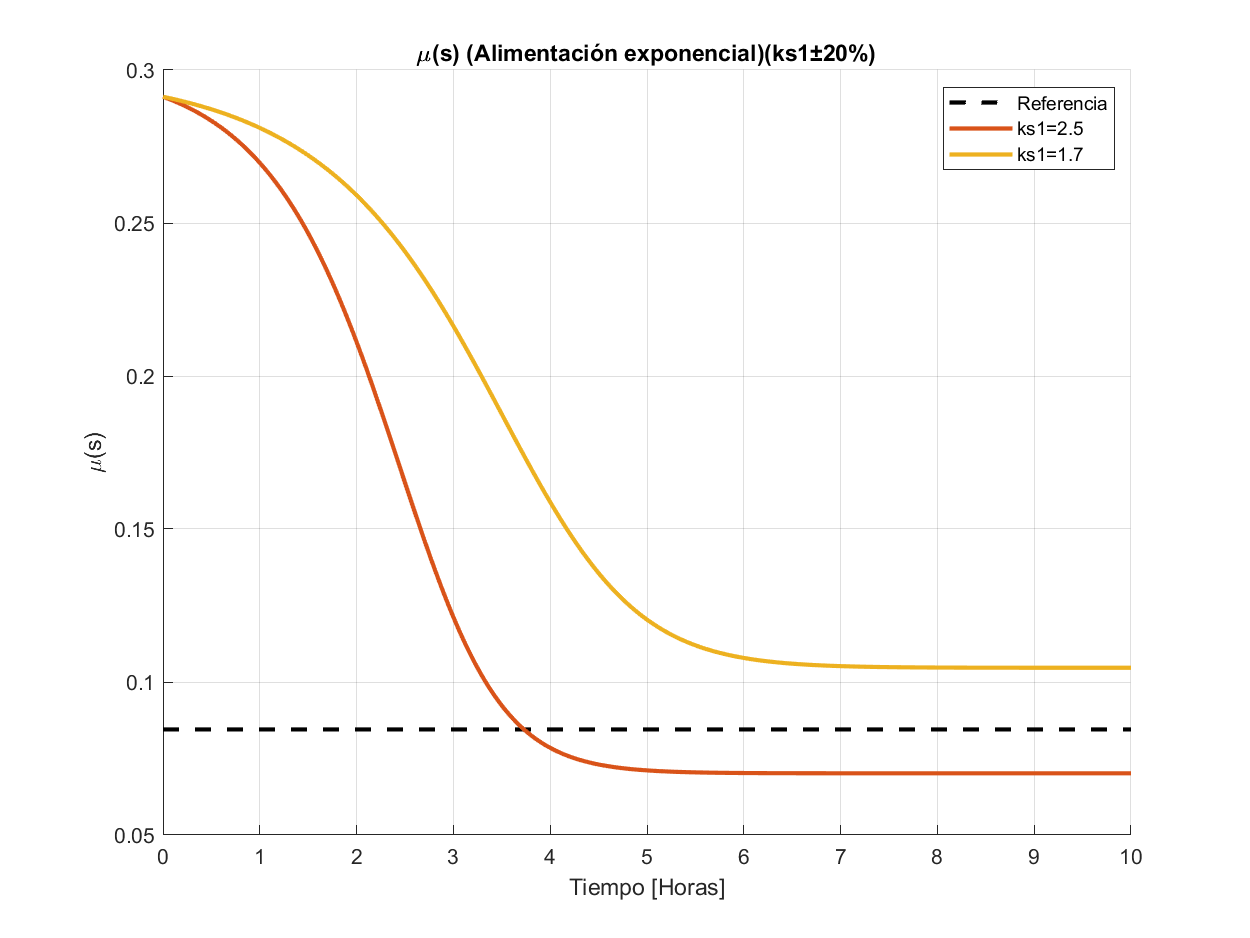
\includegraphics[width=0.43\textwidth]{./Images_tp3/exp_ks1.png}
  \caption{Control con alimentación exponencial (se varía $k_{s1}$)}
\end{figure}
\begin{figure}[H]
  \centering
  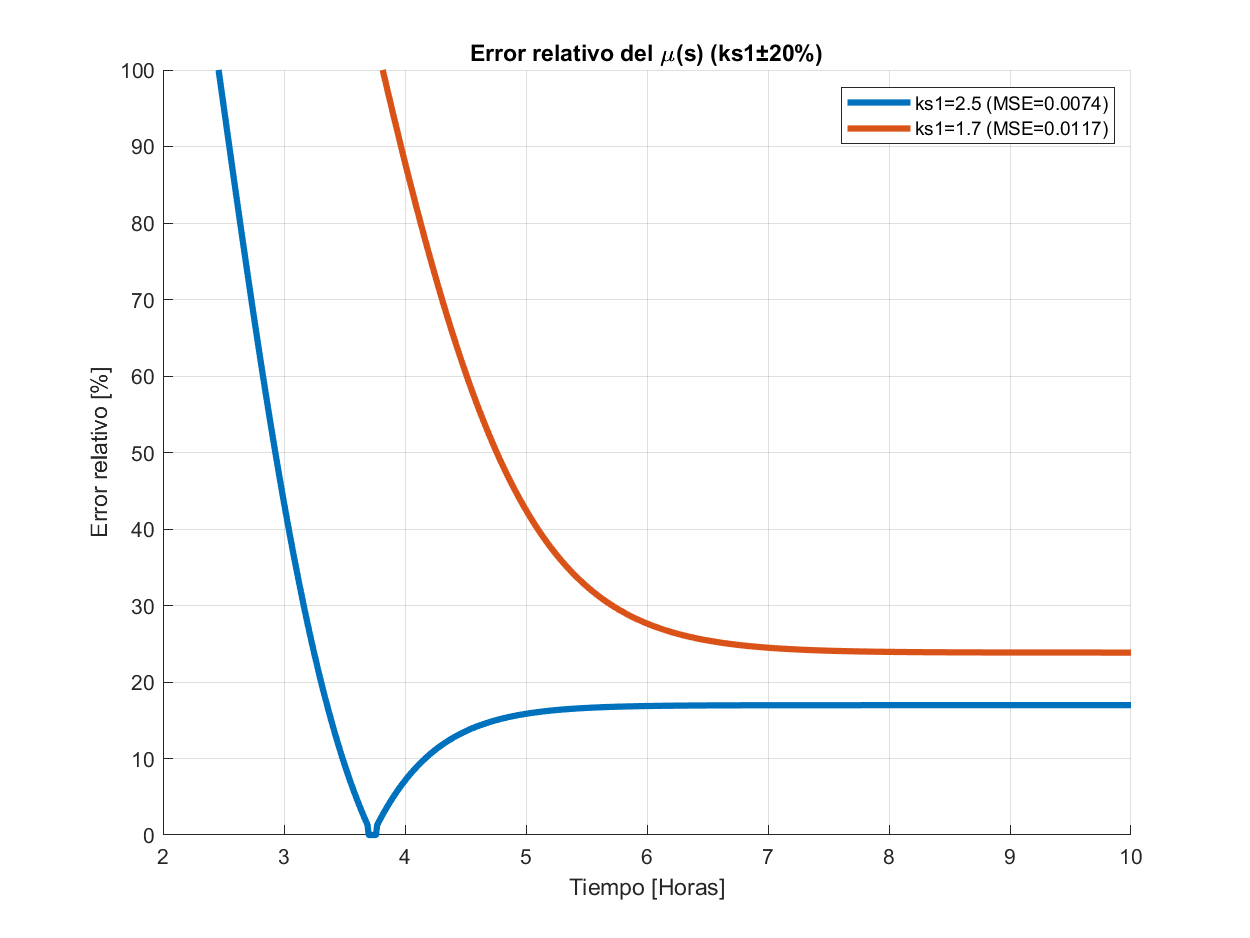
\includegraphics[width=0.43\textwidth]{./Images_tp3/exp_err_ks1.png}
  \caption{Error control con alimentación exponencial (se varía $k_{s1}$)}
\end{figure}

\begin{itemize}  
    \item \(\mu(s)\) converge a un valor distinto al deseado (\(\mu_r(s)\)), con error inicial alto y dinámica lenta.  
    \item \textit{Robustez}: Al variar \(x_0\) y \(k_{s1}\) en \(\pm 20\%\), el error cambia significativamente, indicando baja robustez.  
\end{itemize}  

\subsection{Controlador con acción proporcional (P)}  
Al control anterior se le agrega un término proporcional (\(k_p\)) al error:

\begin{equation}
D = \frac{\mu_r X_0 k_{s1} e^{\mu_r t}}{(s_{\text{in}} - s_r) V} + \frac{k_p (\mu_r - \mu_s)}{(s_{\text{in}} - s_r)}
\end{equation}

\begin{figure}[H]
  \centering
  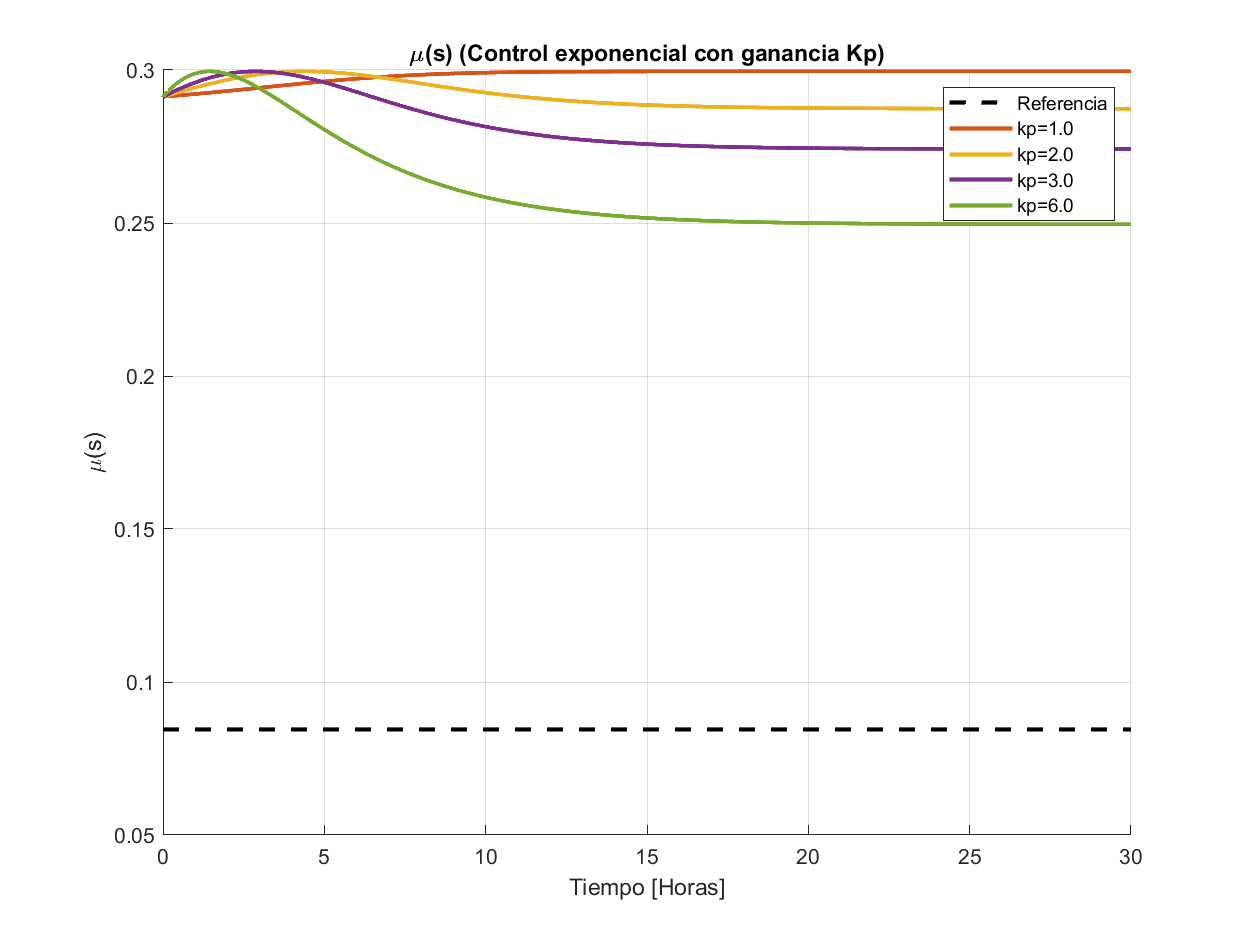
\includegraphics[width=0.43\textwidth]{./Images_tp3/exp_kp.png}
  \caption{Control con alimentación exponencial con término kp}
\end{figure}
\begin{figure}[H]
  \centering
  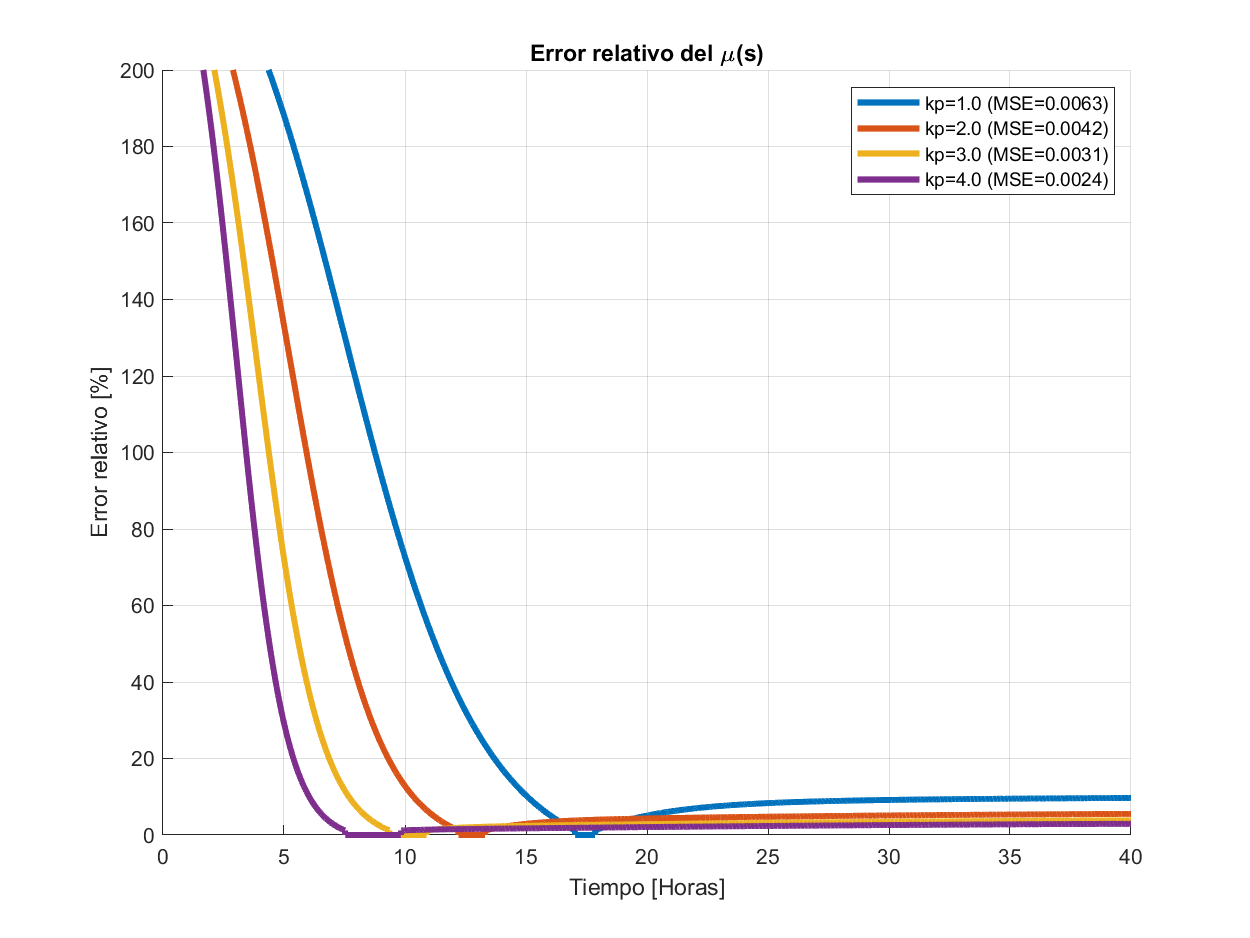
\includegraphics[width=0.43\textwidth]{./Images_tp3/exp_err_kp.png}
  \caption{Error control con alimentación exponencial con término kp}
\end{figure}

\begin{itemize}  
    \item El error disminuye notablemente.  
    \item La convergencia hacia \(\mu_r(s)\) es más rápida y con menor error estacionario.  
\end{itemize}  

\subsection{Controlador con acción proporcional-integral (PI)}  
Al controlador anterior se le incluye otro término que es integral (\(k_i\)):

\begin{equation}
D = \frac{\mu_r X_0 k_{s1} e^{\mu_r t}}{(s_{\text{in}} - s_r) V} + \frac{k_i \int_{0}^{t} e(\tau) \, d\tau + k_p e(t)}{(s_{\text{in}} - s_r)}
\end{equation}

Se probó este controlador con variación de los parámetros $x_0$ y $k_{s1}$ en un $20\%$, además se hizo una perturbación a la acción de control en un $20\%$

\begin{figure}[H]
  \centering
  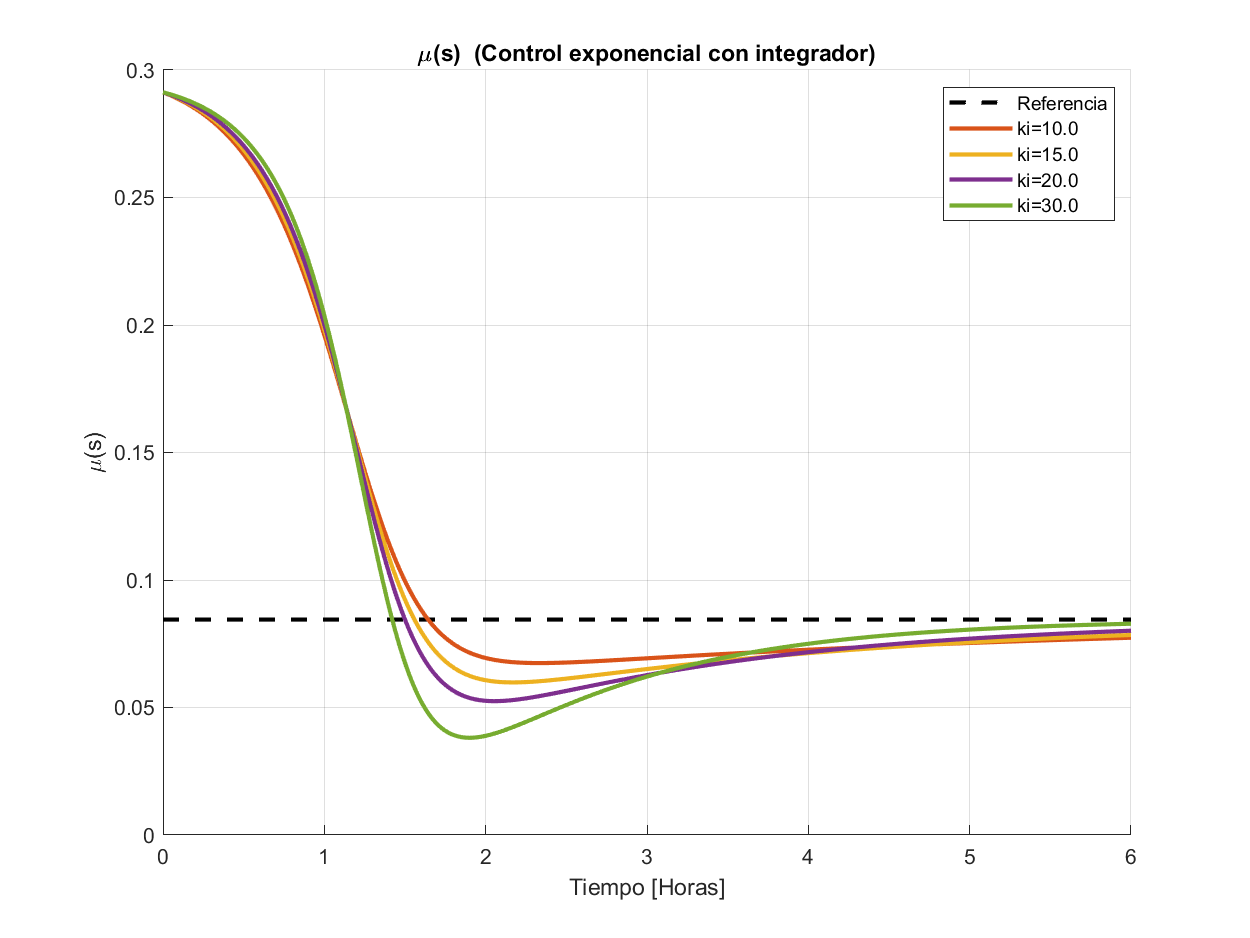
\includegraphics[width=0.43\textwidth]{./Images_tp3/exp_ki.png}
  \caption{Control con alimentación exponencial con términos kp y ki}
\end{figure}
\begin{figure}[H]
  \centering
  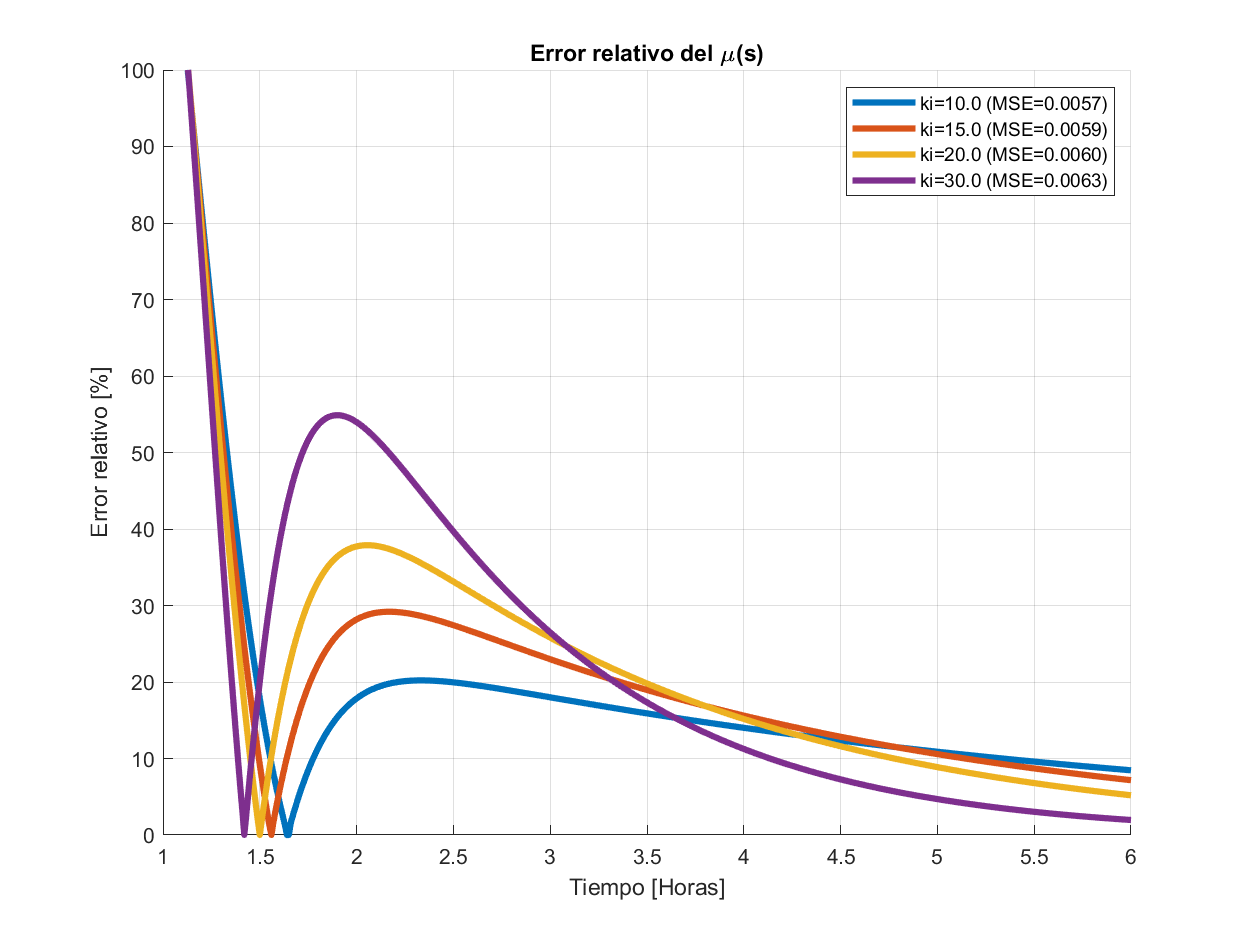
\includegraphics[width=0.43\textwidth]{./Images_tp3/exp_err_ki.png}
  \caption{Error control con alimentación exponencial con términos kp y ki}
\end{figure}

\begin{figure}[H]
  \centering
  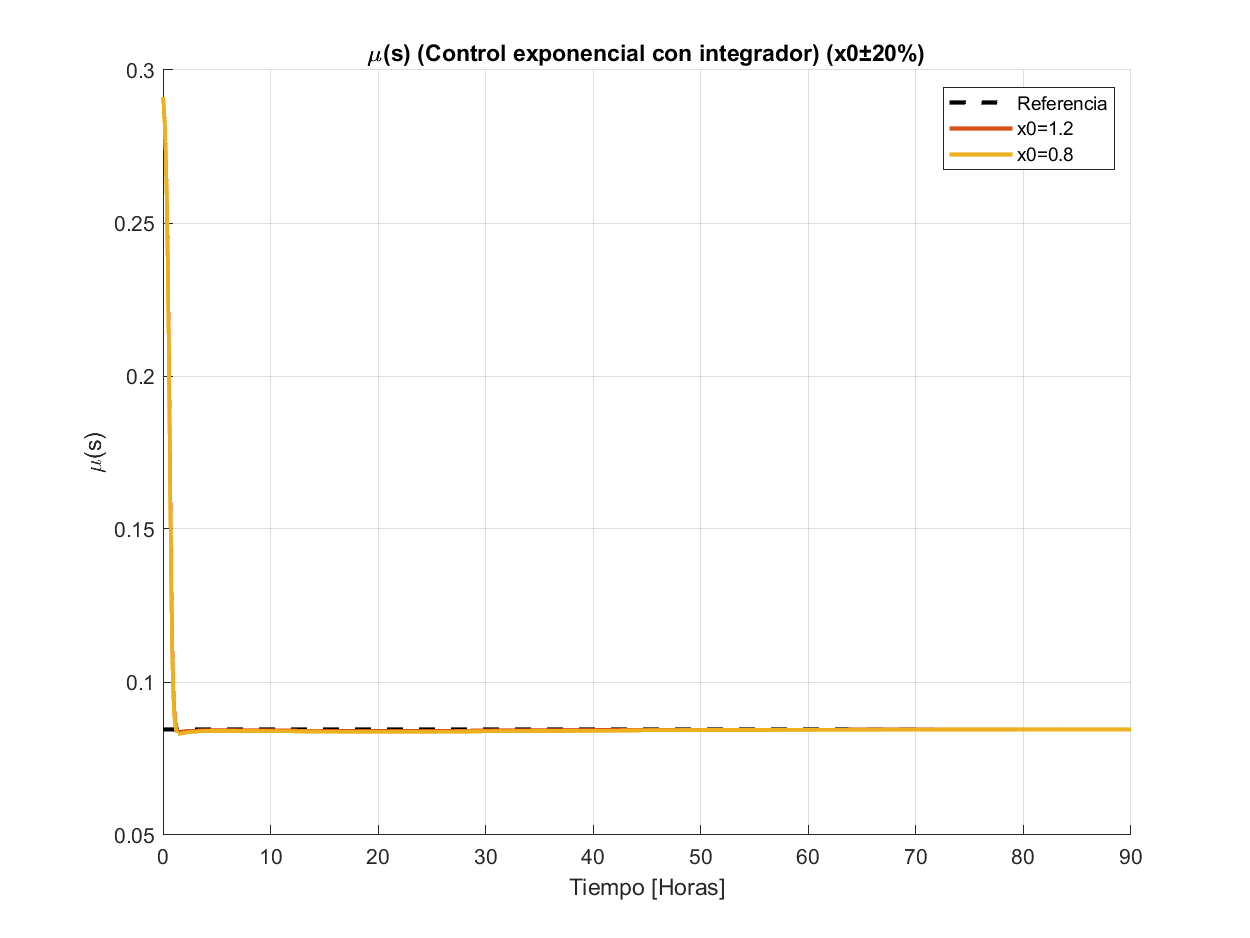
\includegraphics[width=0.43\textwidth]{./Images_tp3/exp_rob_x0.png}
  \caption{Alimentación exponencial (kp y ki) con variaciones en $x_{0}$ }
\end{figure}
\begin{figure}[H]
  \centering
  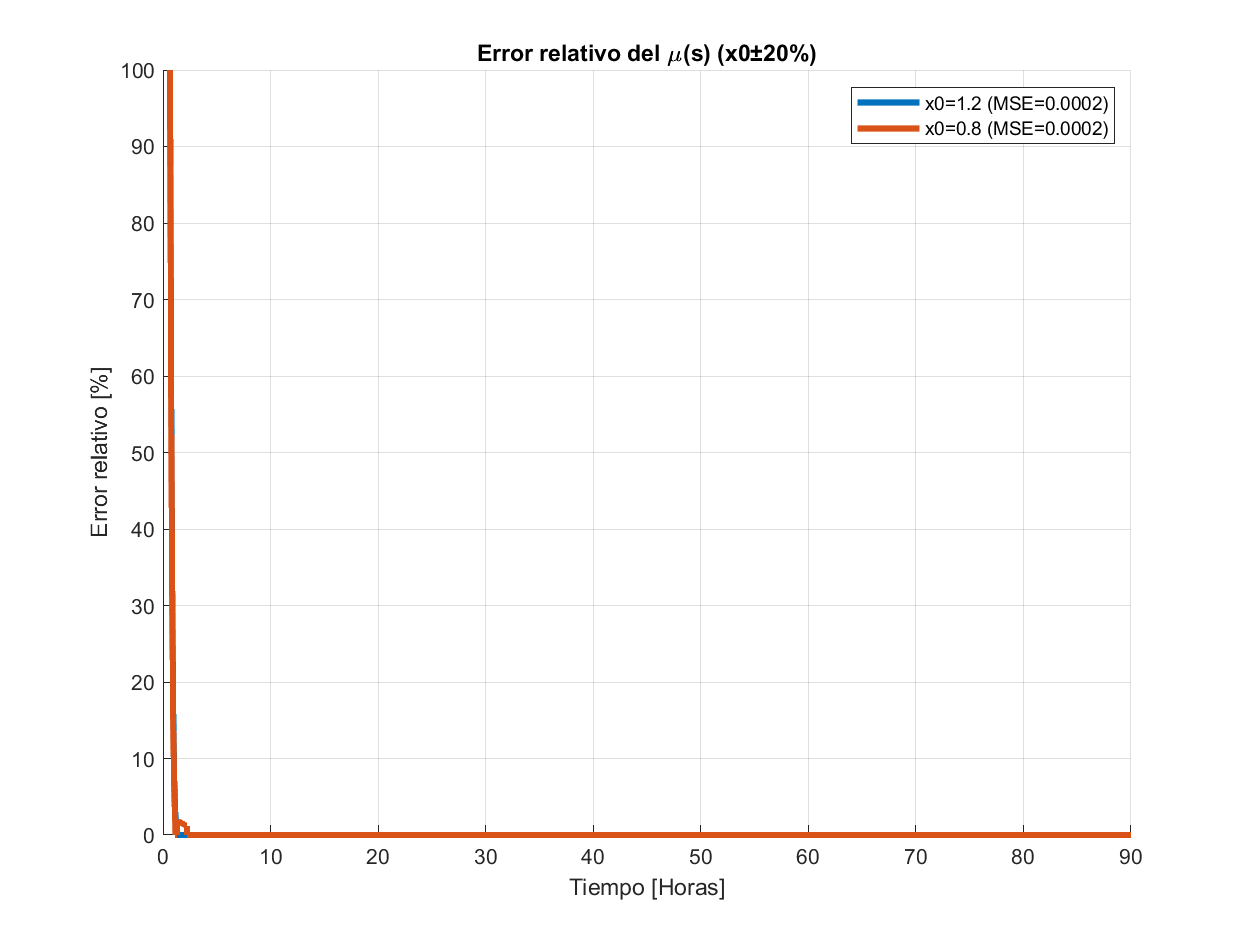
\includegraphics[width=0.43\textwidth]{./Images_tp3/exp_rob_err_x0.png}
  \caption{Error alimentación exponencial (kp y ki) con variaciones en $x_{0}$ }
\end{figure}

\begin{figure}[H]
  \centering
  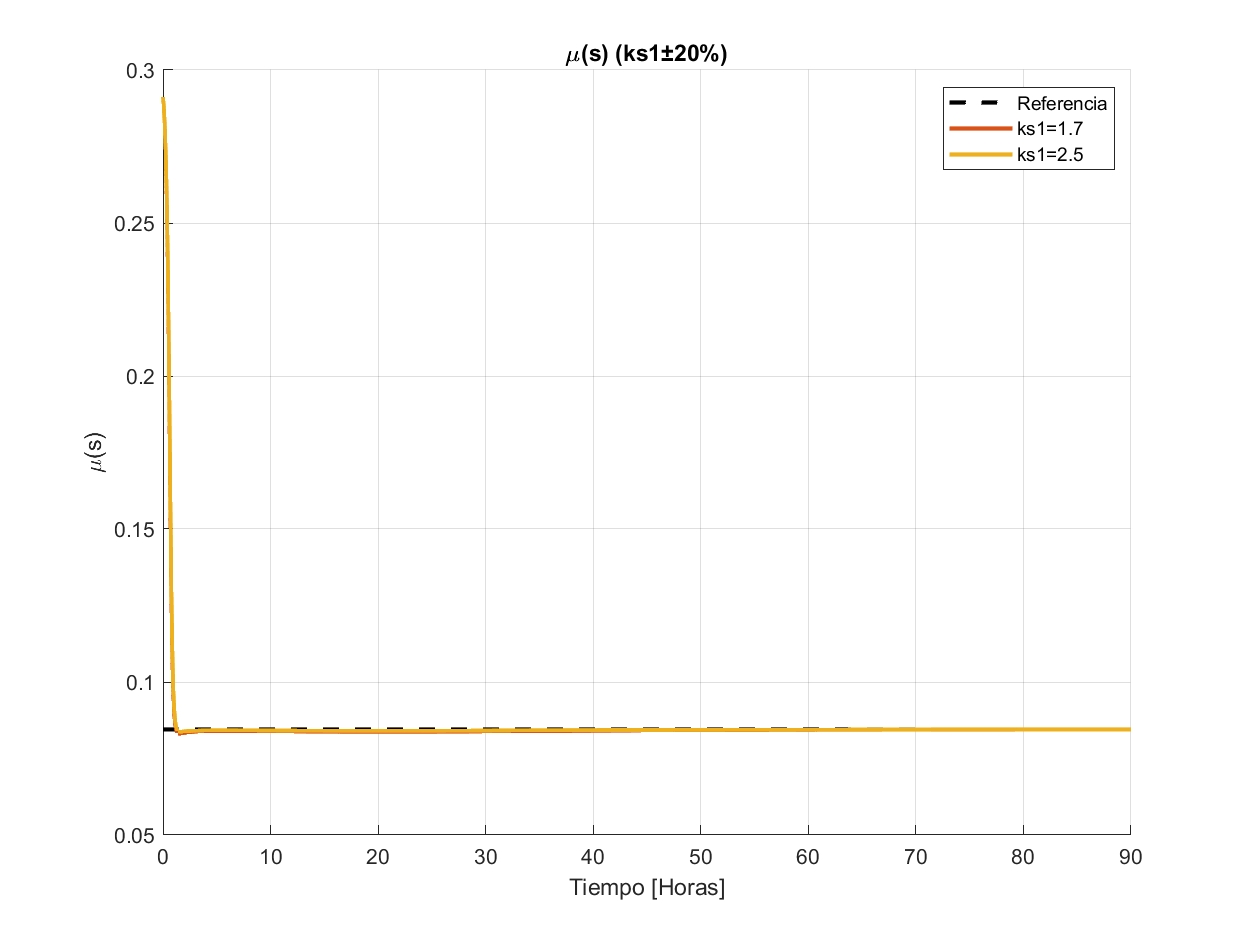
\includegraphics[width=0.43\textwidth]{./Images_tp3/exp_rob_ks1.png}
  \caption{Alimentación exponencial (kp y ki) con variaciones en $k_{s1}$ }
\end{figure}
\begin{figure}[H]
  \centering
  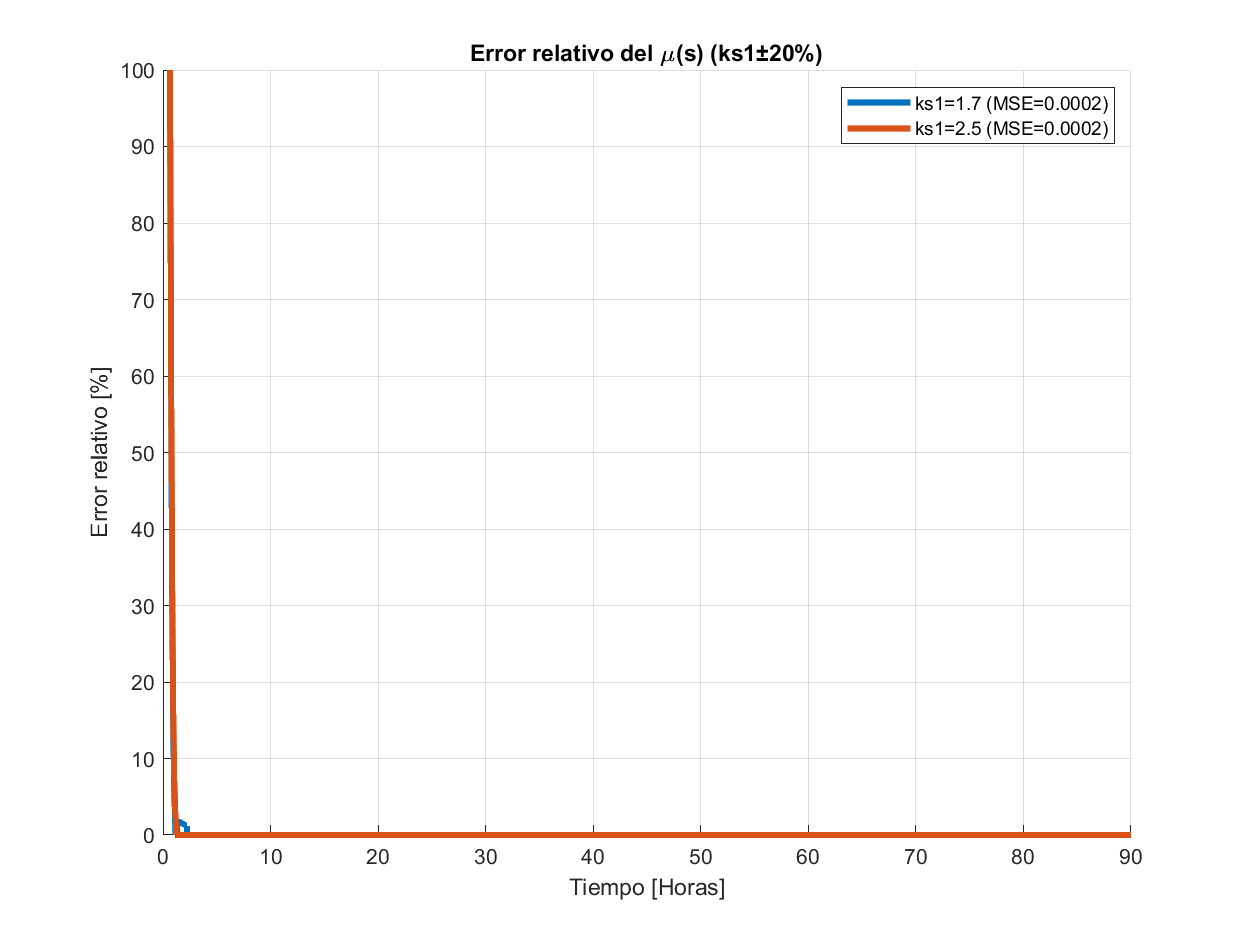
\includegraphics[width=0.43\textwidth]{./Images_tp3/exp_rob_err_ks1.png}
  \caption{Error alimentación exponencial (kp y ki) con variaciones en $k_{s1}$ }
\end{figure}

\begin{figure}[H]
  \centering
  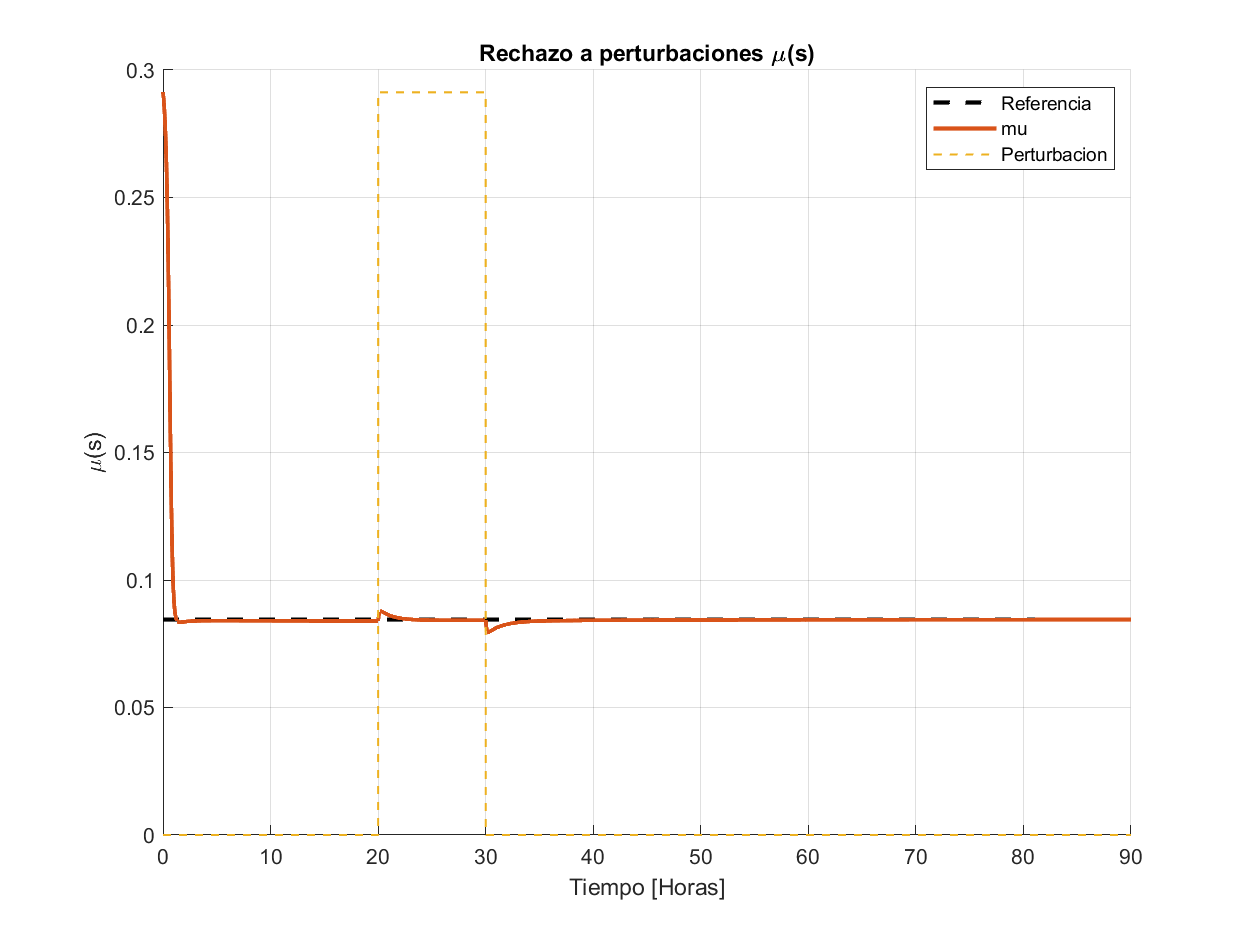
\includegraphics[width=0.43\textwidth]{./Images_tp3/exp_rech.png}
  \caption{Alimentación exponencial (kp y ki) con variaciones en D }
\end{figure}
\begin{figure}[H]
  \centering
  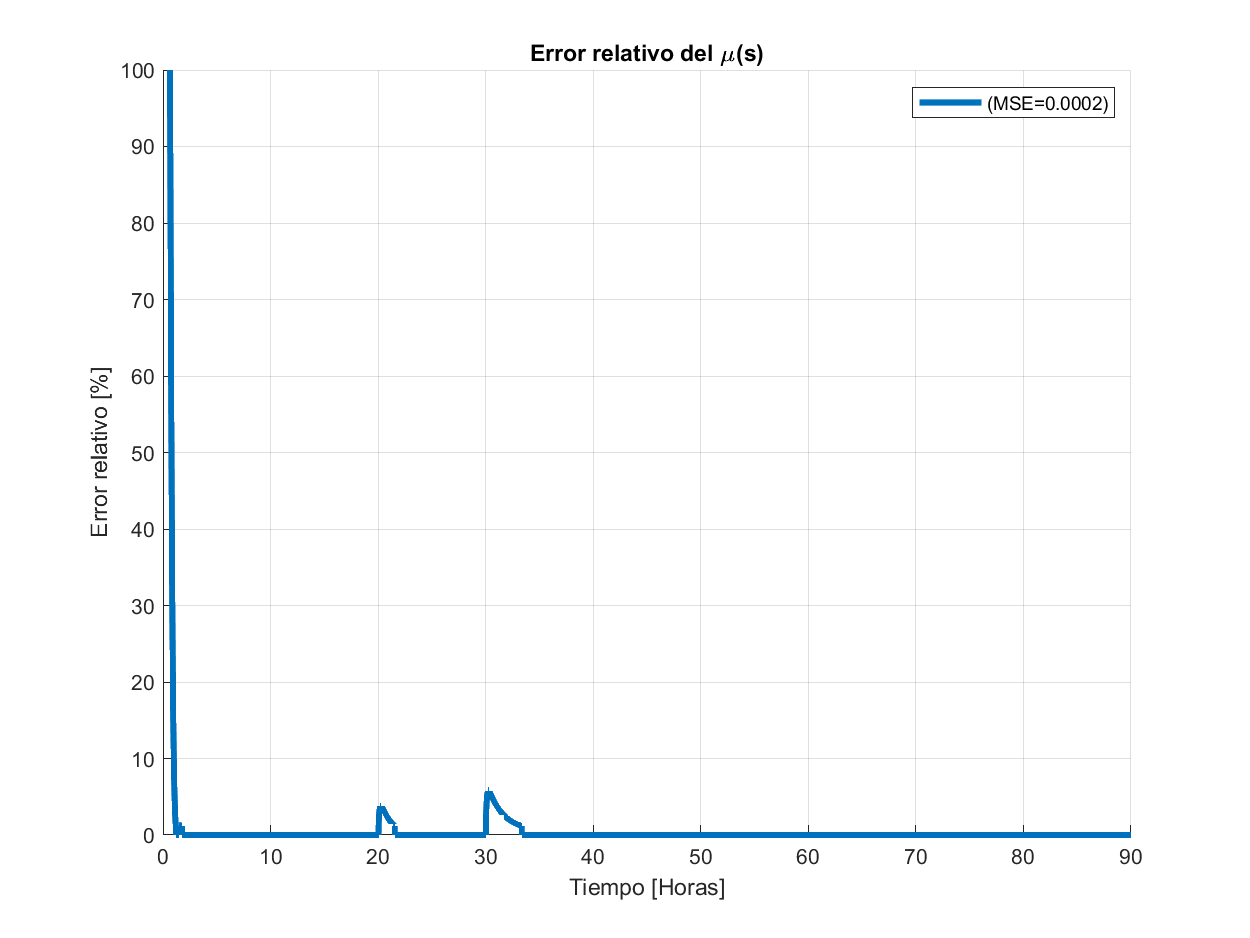
\includegraphics[width=0.43\textwidth]{./Images_tp3/exp_rech_err.png}
  \caption{Error alimentación exponencial (kp y ki) con variaciones en D }
\end{figure}

\begin{itemize}  
    \item \textit{Precisión}: \(\mu(s)\) alcanza \(\mu_r(s)\) en menos de 5 horas, con error nulo.  
    \item \textit{Robustez}: Las variaciones en \(x_0\), \(k_{s1}\), o la acción de control (\(\pm 20\%\)) no afectan el error, demostrando alta robustez.  
\end{itemize}  


\section{Control linealizante del sustrato}  
Se diseña un controlador que cancela la dinámica natural del sustrato, dependiendo únicamente del parámetro \(k_{s1}\) (eliminando la dependencia con \(x_0\)).  

\subsection{Controlador básico (cancelación de dinámica)}

\begin{equation}
D = \frac{\mu_s x k_{s1}}{s_{\text{in}} - s}
\end{equation}

\begin{figure}[h]
  \centering
  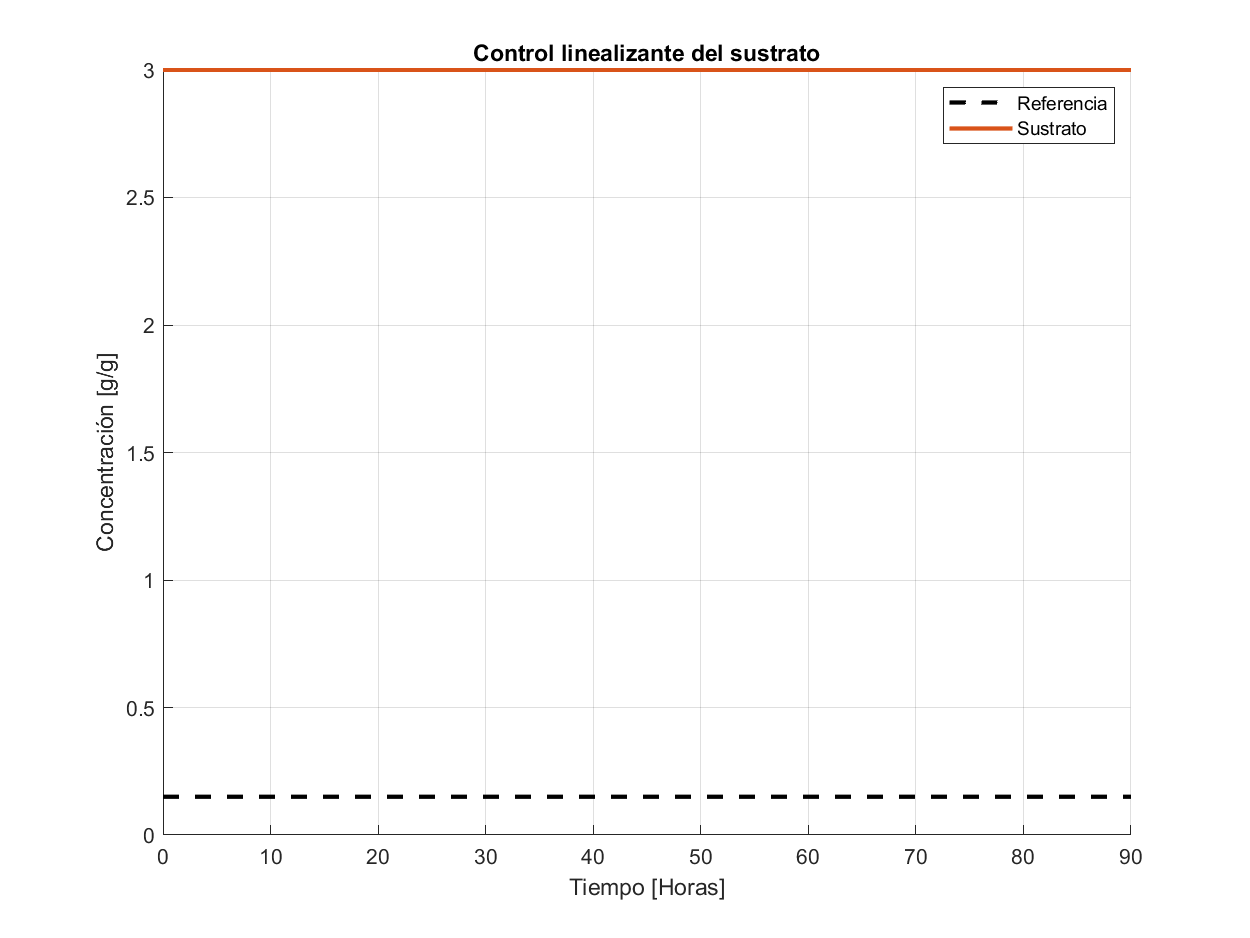
\includegraphics[width=0.43\textwidth]{./images_tp3/lin.png}
  \caption{Control linealizante}
\end{figure}
\begin{figure}[h]
  \centering
  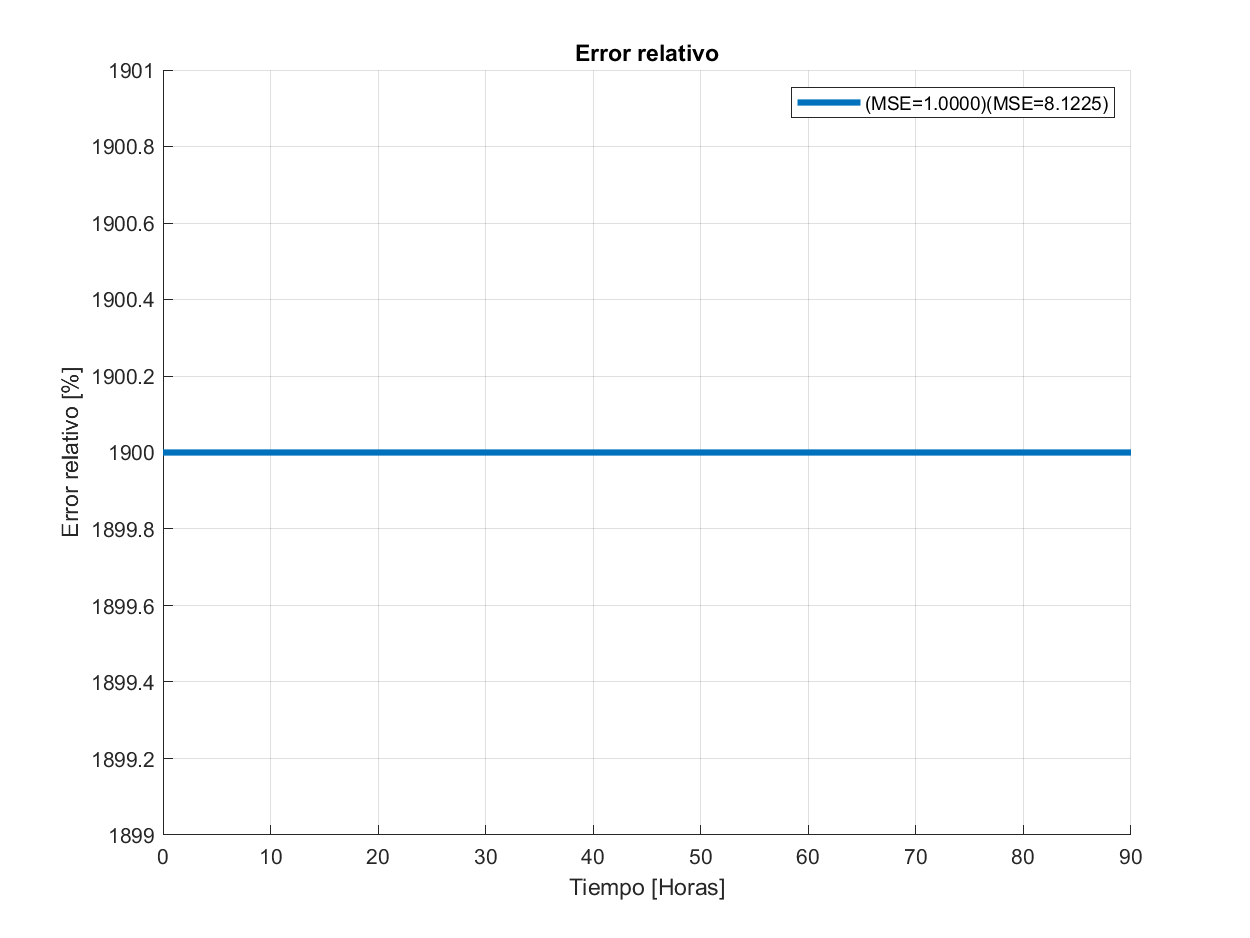
\includegraphics[width=0.43\textwidth]{./images_tp3/lin_err.png}
  \caption{Error control linealizante}
\end{figure}

\begin{figure}[h]
  \centering
  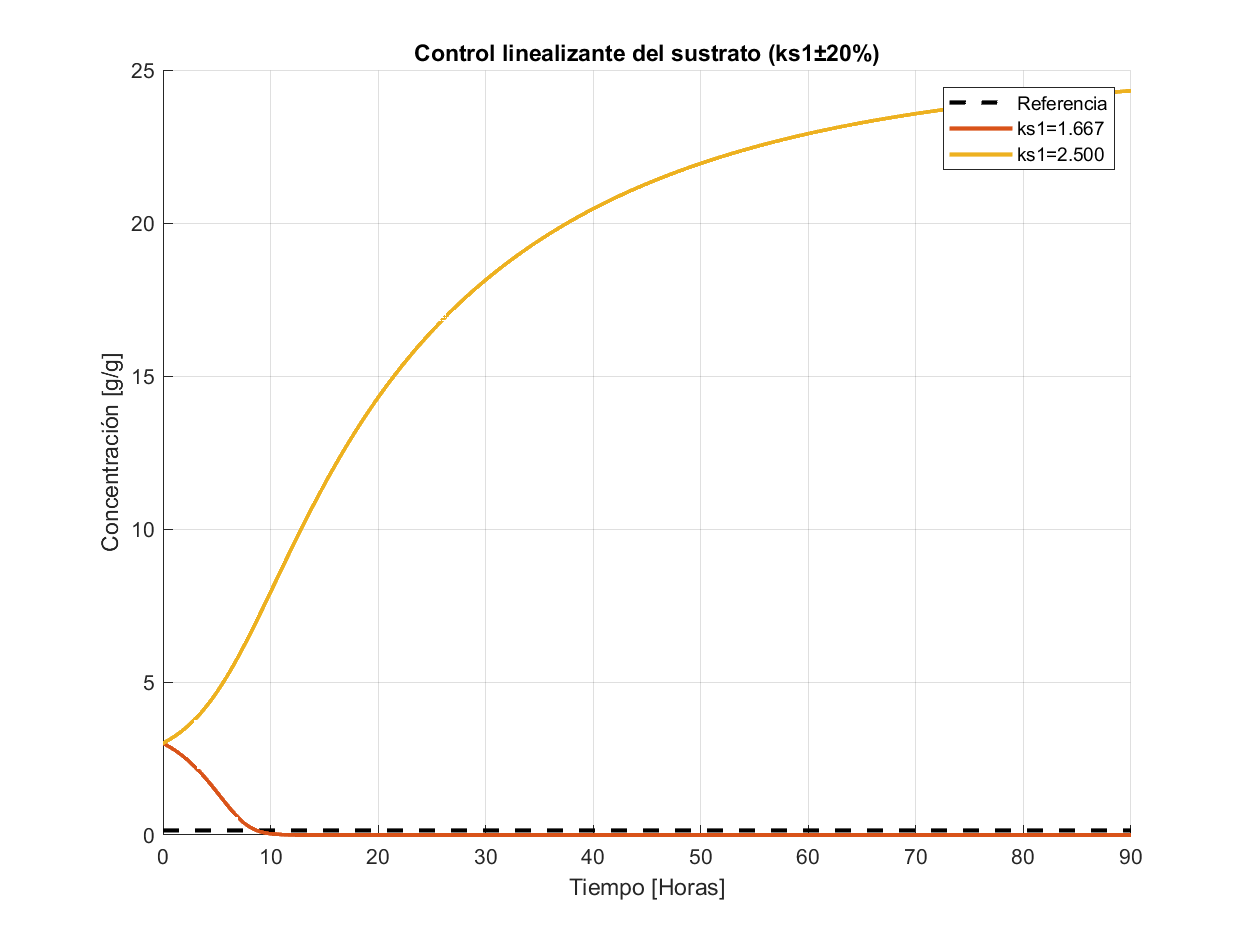
\includegraphics[width=0.43\textwidth]{./images_tp3/lin_ks1.png}
  \caption{Control linealizante con variaciones en $k_{s1}$}
\end{figure}
\begin{figure}[h]
  \centering
  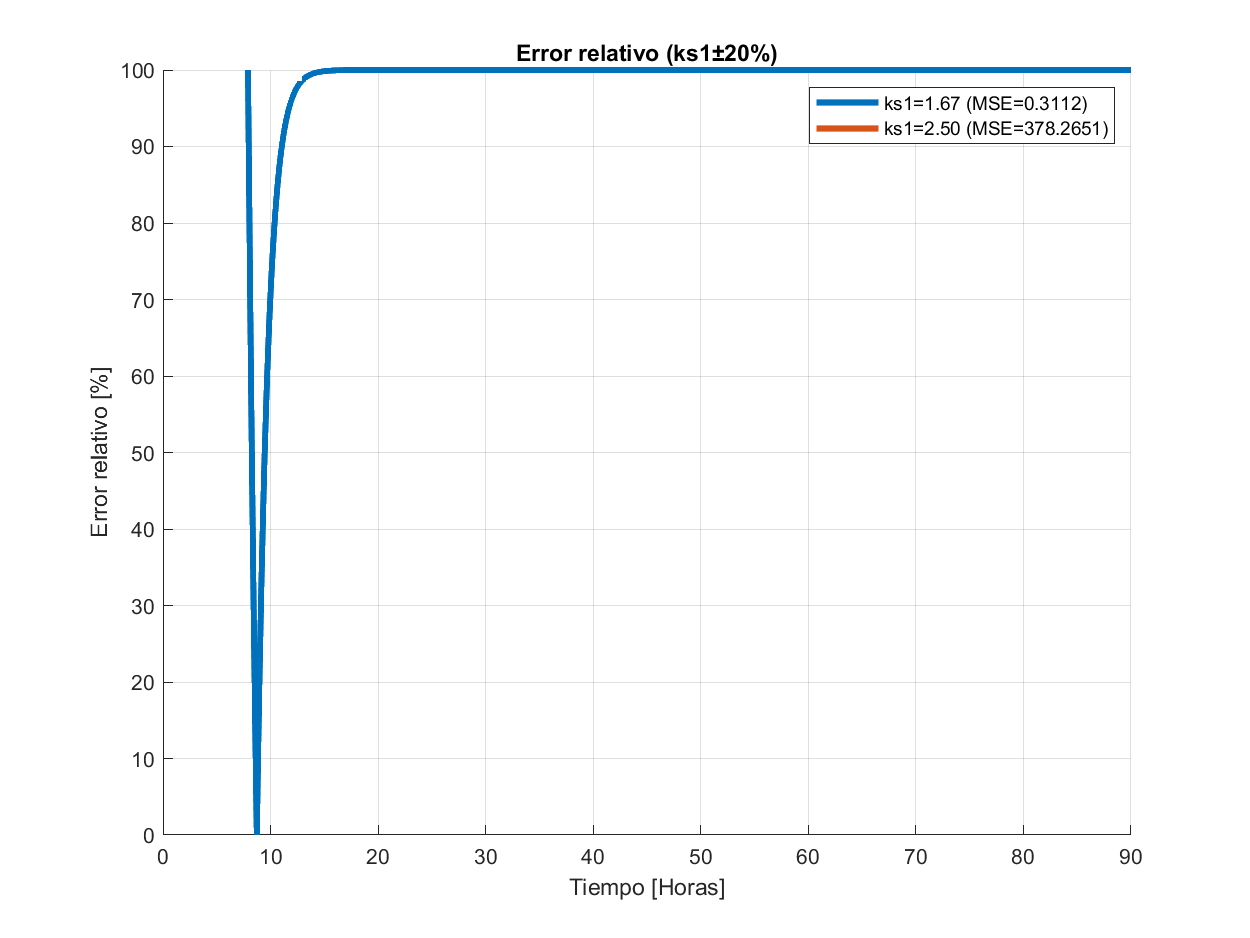
\includegraphics[width=0.43\textwidth]{./images_tp3/lin_err_ks1.png}
  \caption{Error control linealizante con variaciones en $k_{s1}$}
\end{figure}

\begin{itemize}
    \item La dinámica del sustrato es cancelada, pero el error respecto al valor de referencia es significativo, como es de esperar.  
    \item \textit{Sensibilidad al modelo}: Al variar \(k_{s1}\) en \(\pm 20\%\), el sistema muestra comportamientos inestables (incluso divergencia), evidenciando alta dependencia del modelo exacto.  
\end{itemize}  

\subsection{Inclusión de acción proporcional (P)}  
Para solucionar todos los problemas anteriores se añade un término proporcional al error (ganancia \(k_p\)):  

\begin{equation}
D = \frac{\mu_s(t) x(t) k_{s1} + k_p [s_r - s(t)]}{s_{\text{in}} - s_r}
\end{equation}

\begin{figure}[H]
  \centering
  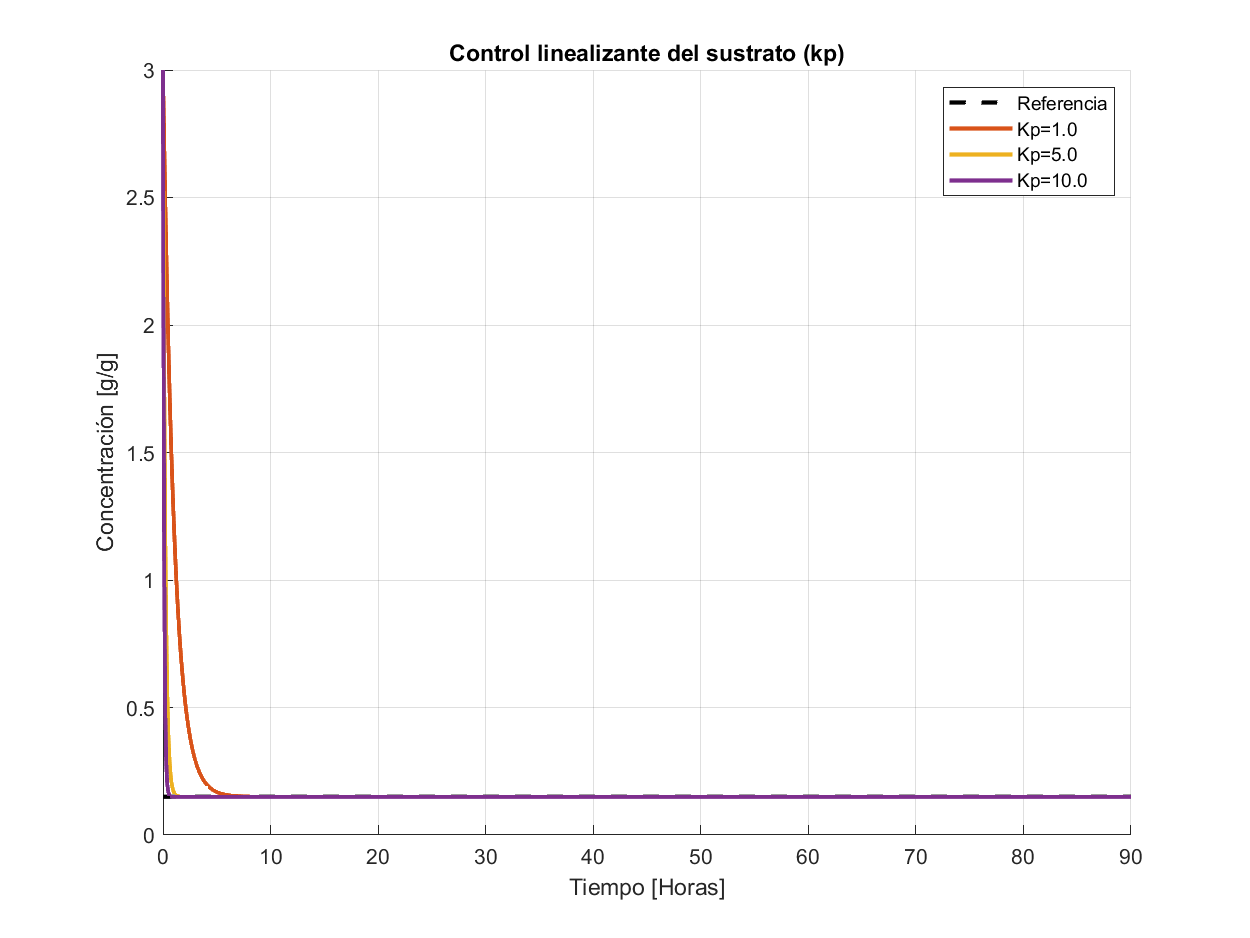
\includegraphics[width=0.43\textwidth]{./Images_tp3/lin_kp.png}
  \caption{Control linealizante con término proporcional}
\end{figure}
\begin{figure}[H]
  \centering
  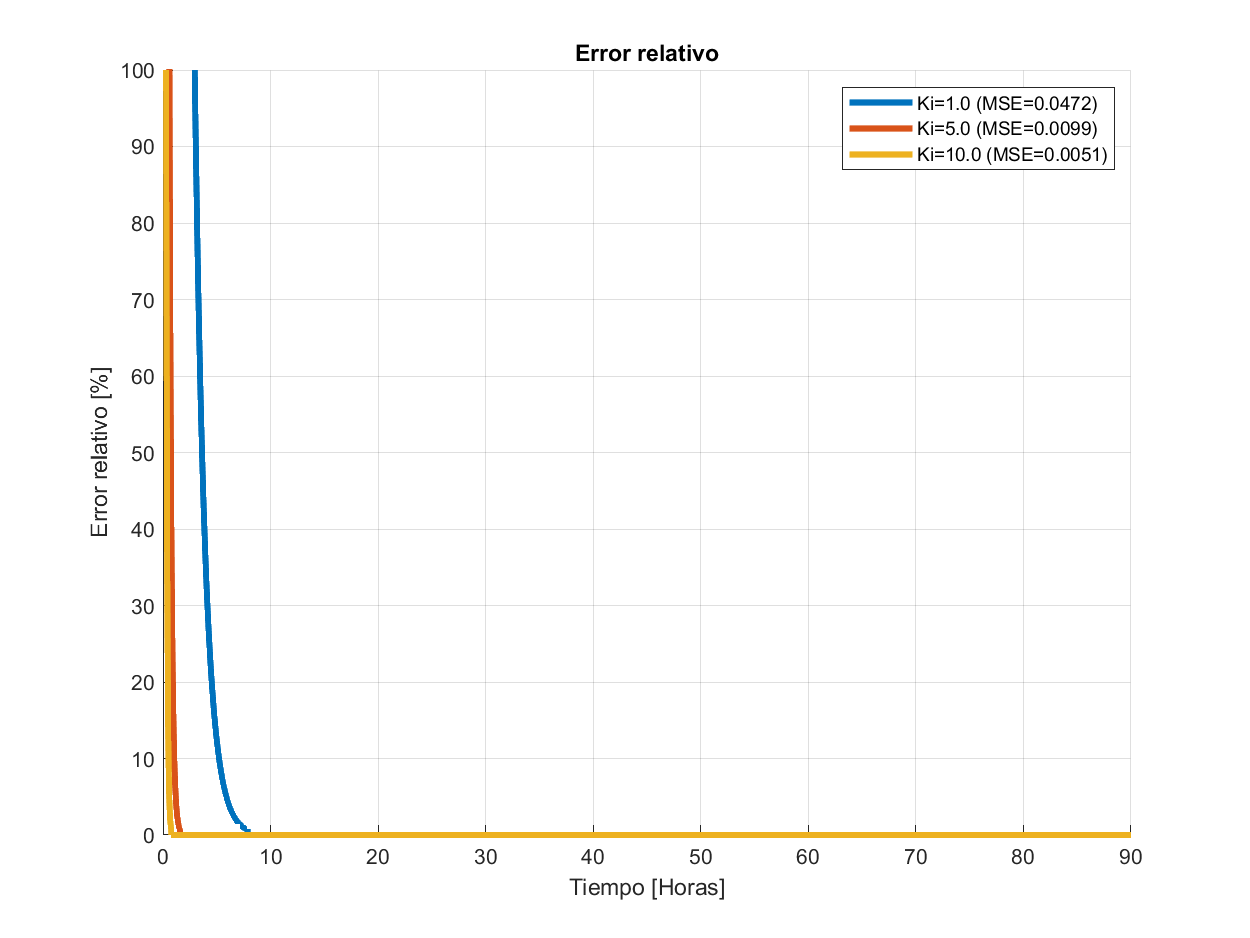
\includegraphics[width=0.43\textwidth]{./Images_tp3/lin_kp_err.png}
  \caption{Error control linealizante con término proporcional}
\end{figure}

\begin{figure}[H]
  \centering
  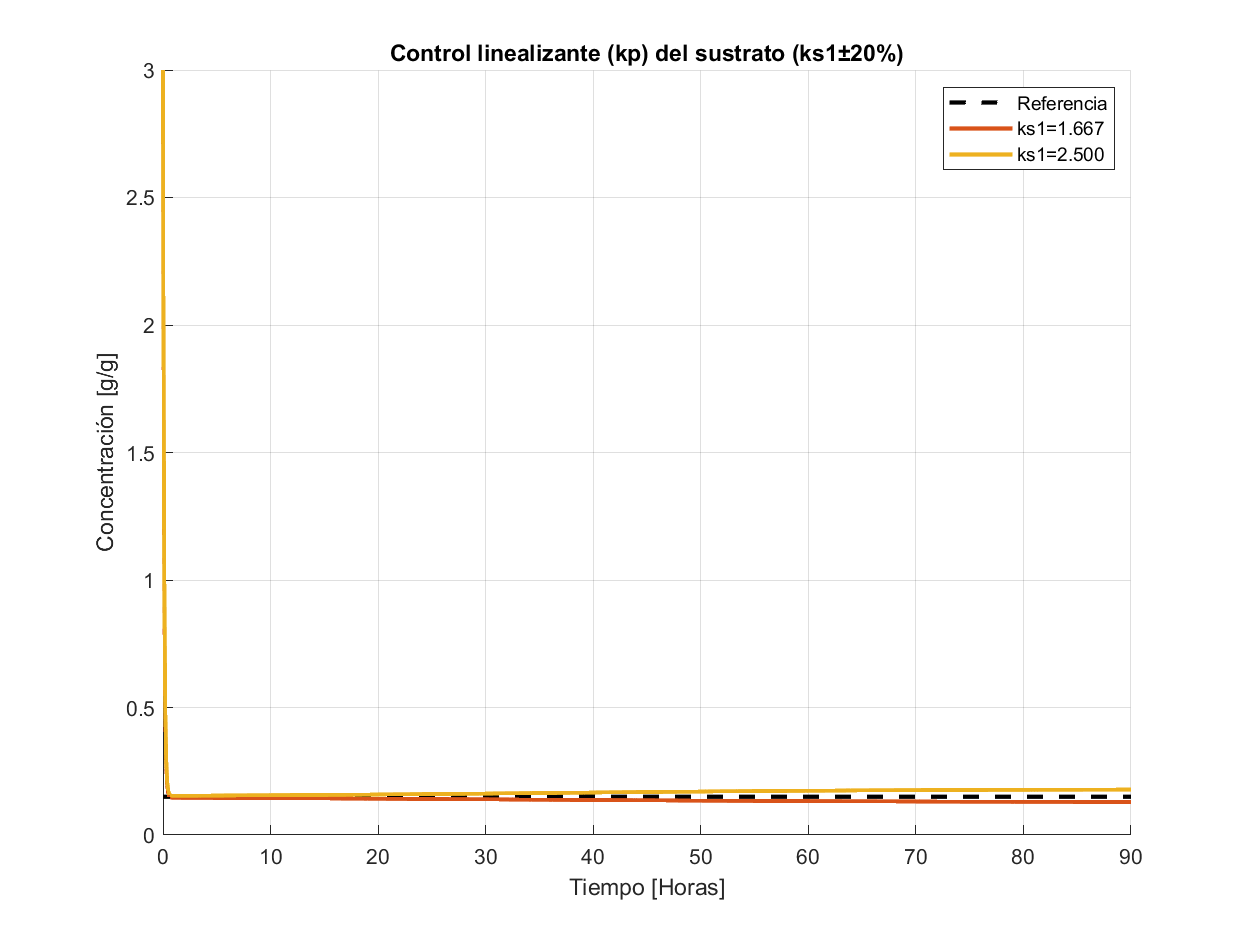
\includegraphics[width=0.43\textwidth]{./Images_tp3/lin_kp_ks1.png}
  \caption{Control linealizante con término proporcional y variaciones en $k_{s1}$}
\end{figure}
\begin{figure}[H]
  \centering
  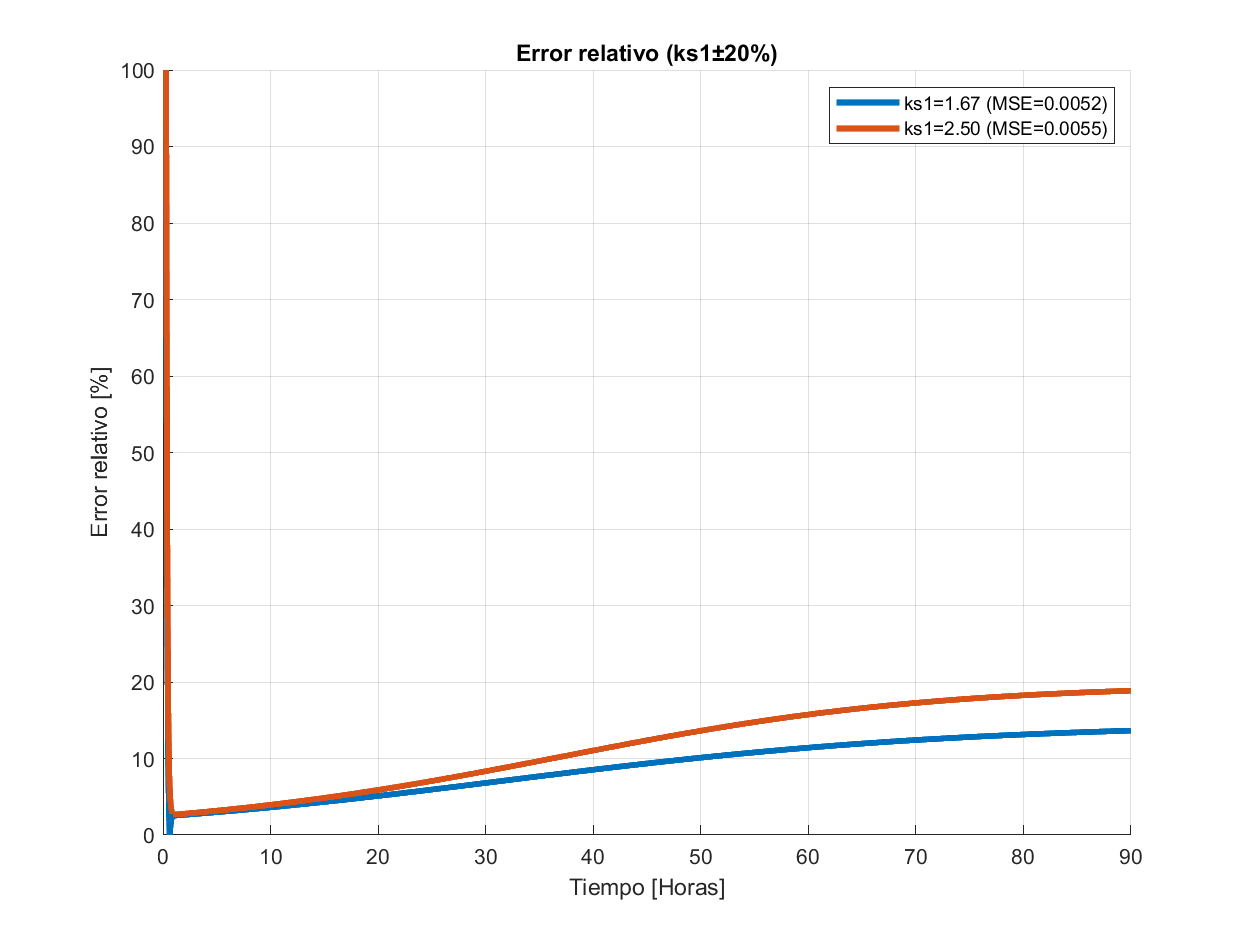
\includegraphics[width=0.43\textwidth]{./Images_tp3/lin_kp_err_ks1.png}
  \caption{Error control linealizante con término proporcional y variaciones en $k_{s1}$}
\end{figure}

\begin{itemize}  
    \item \textit{Precisión}: El sistema alcanza la referencia en menos de 3 horas, sin error en estado estacionario.  
    \item \textit{Simplicidad}: No se requiere acción integrativa para eliminar el error.  
    \item \textit{Robustez limitada}: Variaciones del \(20\%\) en \(k_{s1}\) generan error estacionario.
\end{itemize}  

\subsection{Inclusión de acción integral (PI)}  
Se añade un término integral (ganancia \(k_i\)), para disminuir la ganacia \(k_p\) sin perder los beneficios, y además eliminar el error al estado estacionario.

\begin{equation}
D = \frac{\mu_s x k_{s1}}{s_{\text{in}} - s_r} + \frac{k_p e(t) + k_i \int_{0}^{t} e(\tau) \, d\tau}{s_{\text{in}} - s_r}
\end{equation}

\begin{figure}[H]
  \centering
  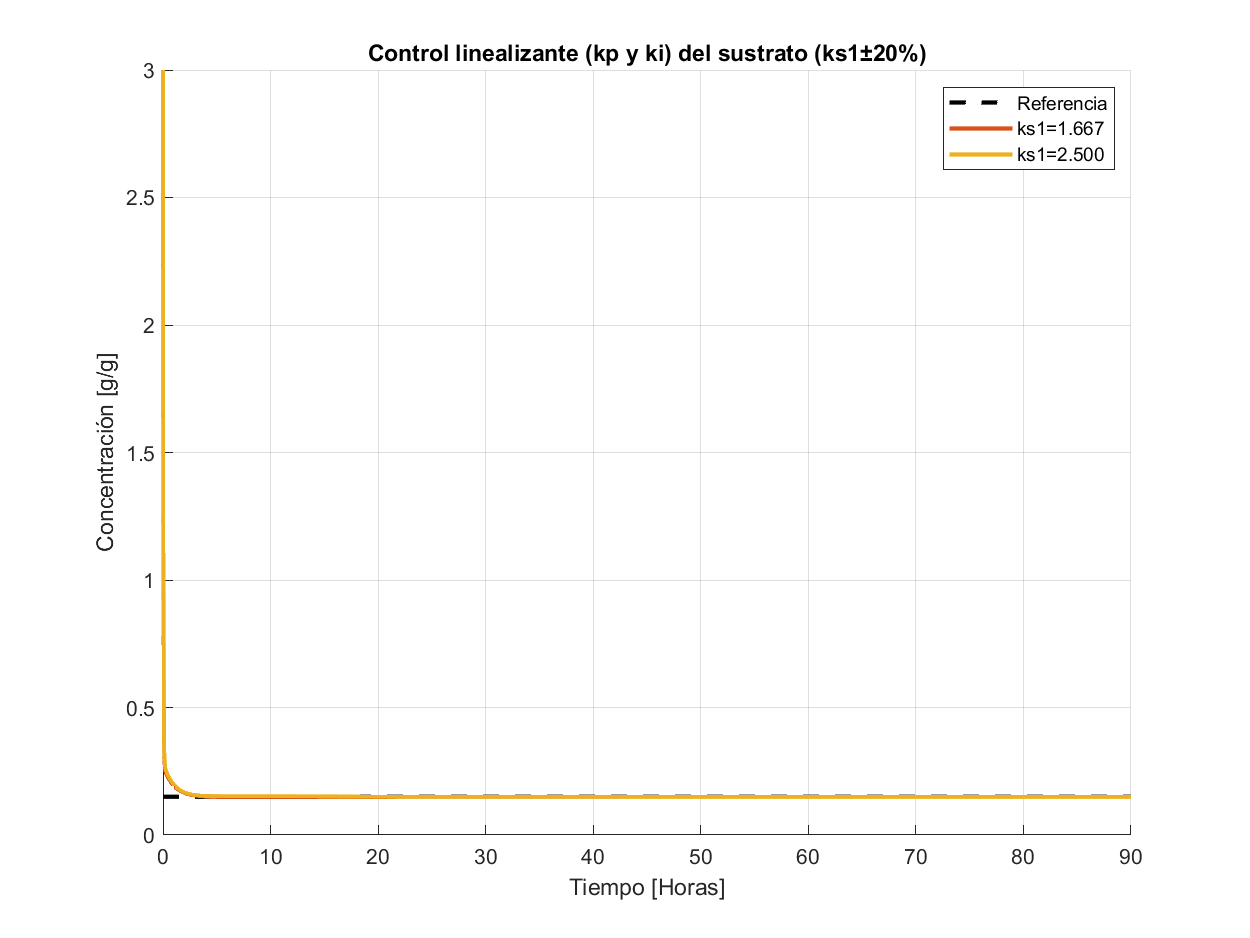
\includegraphics[width=0.43\textwidth]{./Images_tp3/lin_ki.png}
  \caption{Control linealizante proporcional e integrativo}
\end{figure}
\begin{figure}[H]
  \centering
  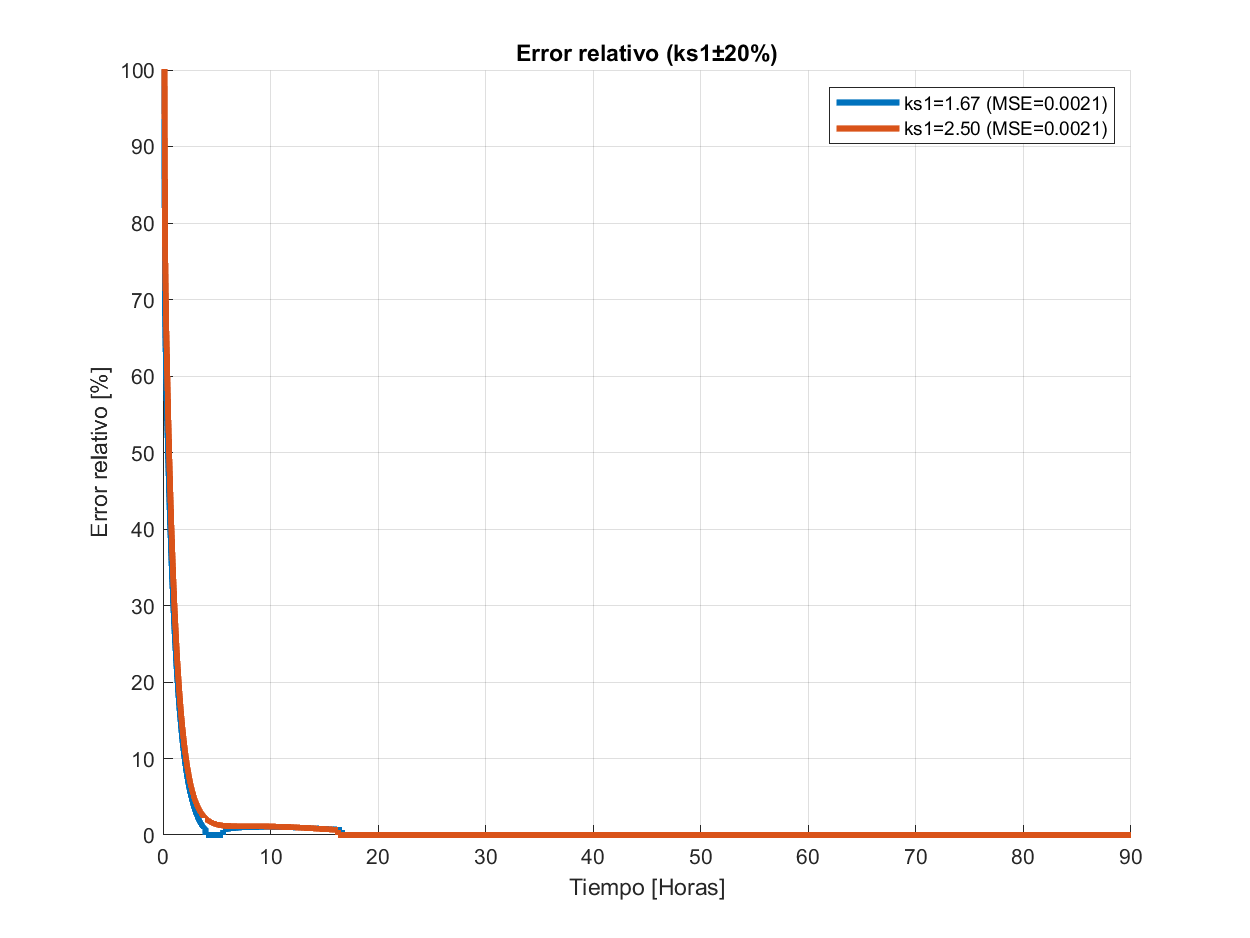
\includegraphics[width=0.43\textwidth]{./Images_tp3/lin_ki_err.png}
  \caption{Error control linealizante proporcional e integrativo}
\end{figure}

\begin{figure}[H]
  \centering
  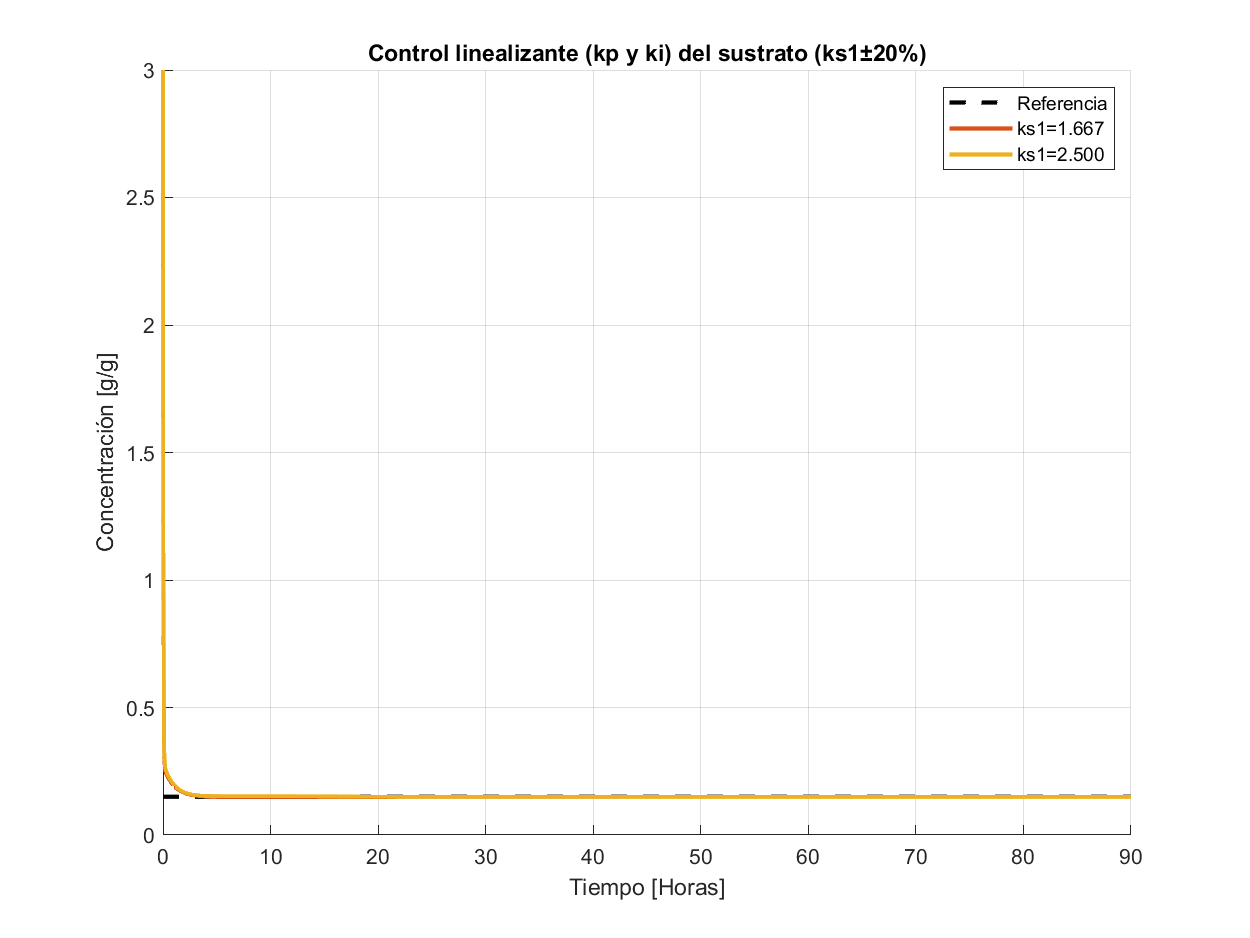
\includegraphics[width=0.43\textwidth]{./Images_tp3/lin_ki.png}
  \caption{Control linealizante proporcional e integrativo con variaciones en $k_{s1}$}
\end{figure}
\begin{figure}[H]
  \centering
  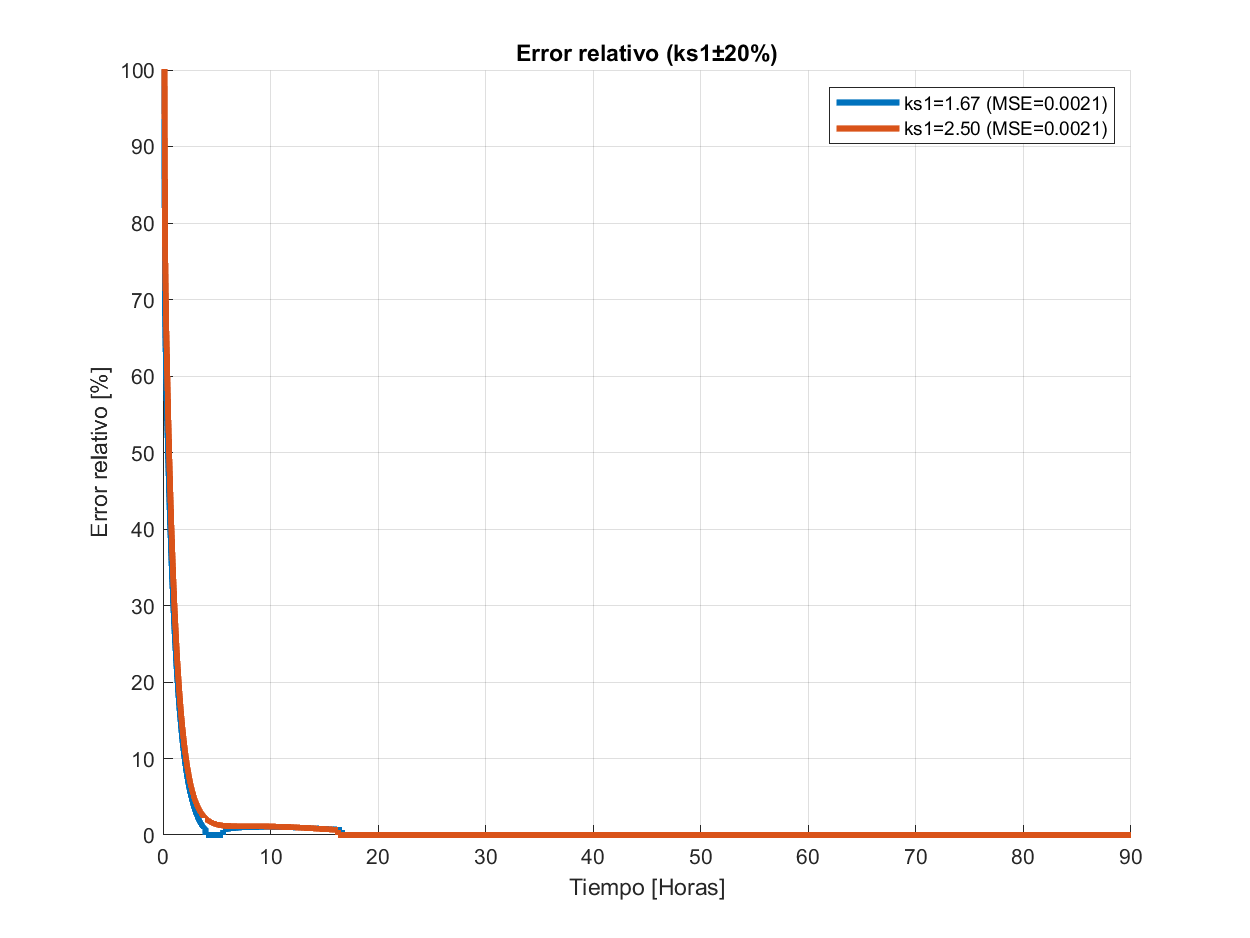
\includegraphics[width=0.43\textwidth]{./Images_tp3/lin_ki_err.png}
  \caption{Error control linealizante proporcional e integrativo con variaciones en $k_{s1}$}
\end{figure}

\begin{itemize}  
    \item \textit{Error nulo}: Aun con variaciones en \(k_{s1}\), el error en estado estacionario es eliminado.  
    \item \textit{Dinámica rápida}: Convergencia en menos de 20 horas (ajustable mediante \(k_p\) y \(k_i\)).  
    \item \textit{Estabilidad}: Ganancias altas mejoran la velocidad pero pueden desestabilizar el sistema, requiriendo sintonización cuidadosa.  
\end{itemize}  

\section{Control Adaptivo}

Se implementó un control adaptivo basado en la metodología vista en clase, el cual resulta similar en estructura a los controladores previos con término integrativo, pero con ventajas significativas en términos sistematicidad para su diseño.

\begin{equation*}
D(t) = \frac{k_{s1} x(t) \hat{\mu}(t) + \gamma_1 [s_r - s(t)]}{s_{\text{in}} - s_r}
\end{equation*}

\begin{equation*}
\frac{d\hat{\mu}(t)}{dt} = \gamma_1 k_{s1} x(t) [s_r - s(t)]
\end{equation*}

\subsection{Comportamiento del Controlador}

\begin{figure}[H]
  \centering
  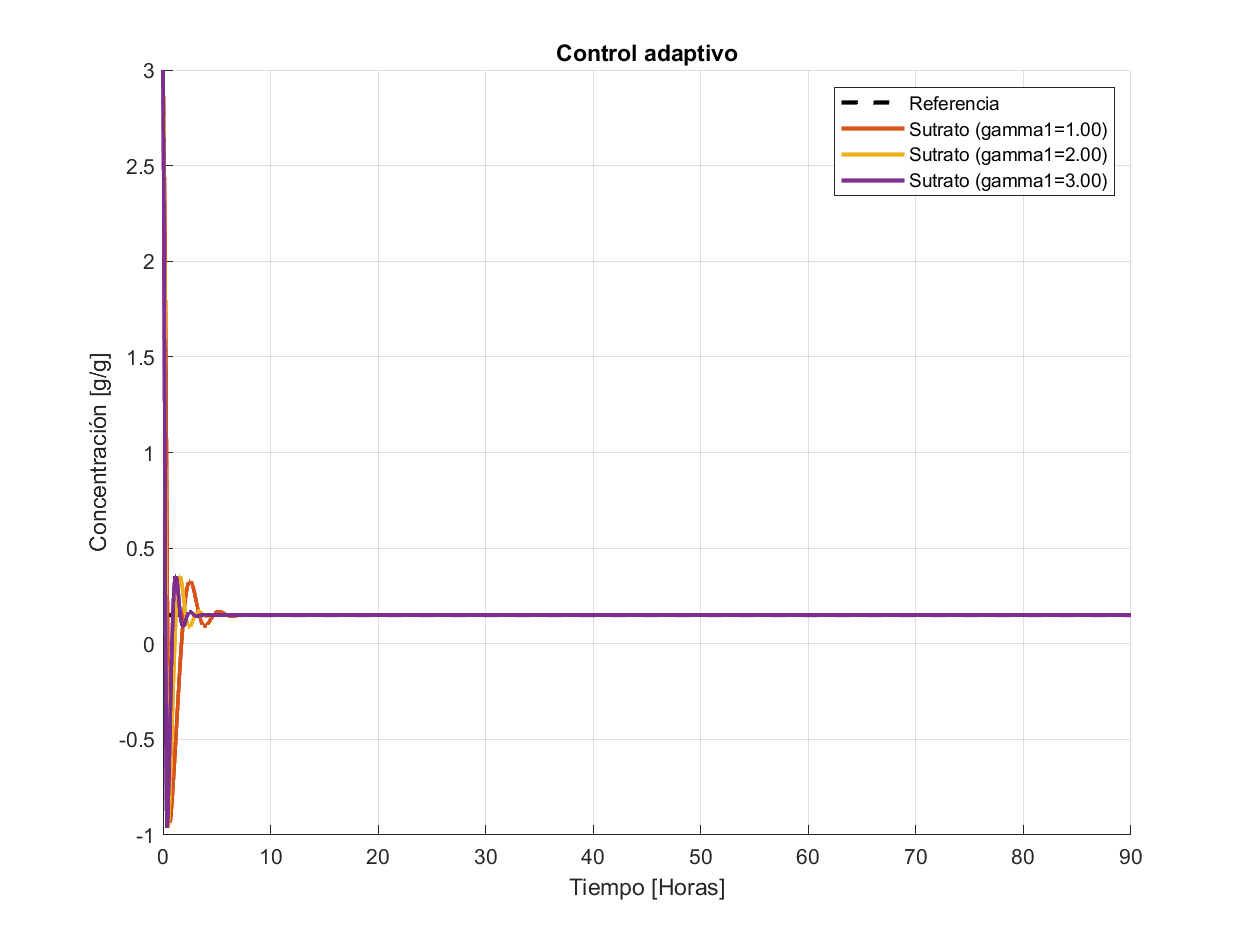
\includegraphics[width=0.43\textwidth]{./Images_tp3/ad.png}
  \caption{Control adaptivo para diferentes valores de $\gamma$}
\end{figure}
\begin{figure}[H]
  \centering
  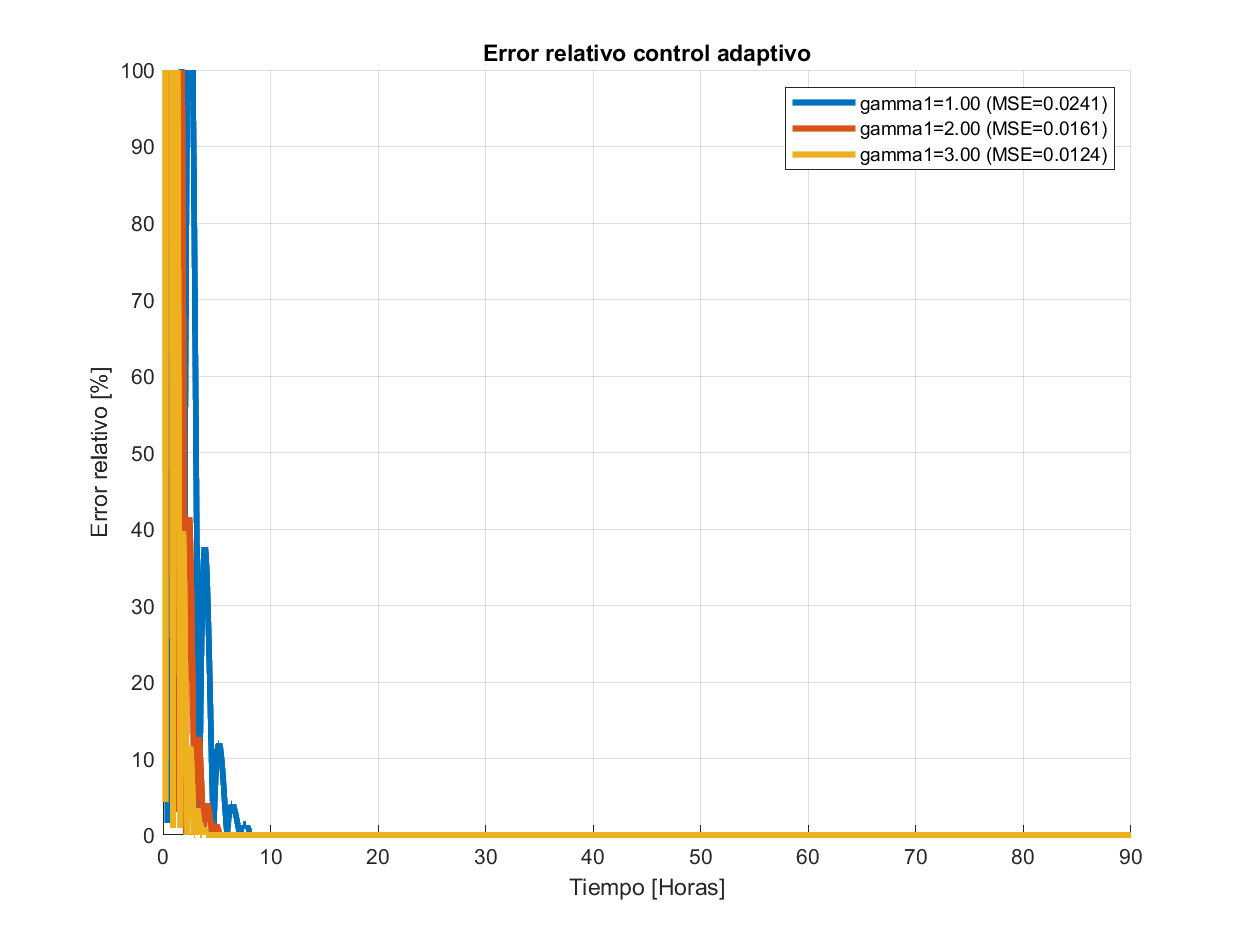
\includegraphics[width=0.43\textwidth]{./Images_tp3/ad_err.png}
  \caption{Error control adaptivo para diferentes valores de $\gamma$}
\end{figure}

\begin{itemize}
    \item \textit{Dinámica inicial}: Presenta mayores oscilaciones al inicio comparado con los controladores anteriores, pero logra converger a error de estado estacionario nulo.
    \item \textit{Tiempo de estabilización}: Las oscilaciones se atenúan antes de las 10 horas (5 horas para \(\gamma = 3\)), demostrando que el parámetro \(\gamma\) permite ajustar la velocidad de convergencia y la amplitud de las oscilaciones iniciales.
    \item \textit{Ventaja clave}: A diferencia de los controladores PI convencionales, este método no requiere conocimiento detallado del modelo del sistema y sigue un enfoque más sistemático.
\end{itemize}

\subsection{Análisis de Robustez}

Se prueba la robustez del controlador variando $k_{s1}$ en un $20\%$, también introduciendo una perturbanción en la acción de control D, variandola en un $20\%$; y finalmente se verifica el correcto funcionamiento considerando el modelo completo y los modelos cinéticos completos también.

\begin{figure}[H]
  \centering
  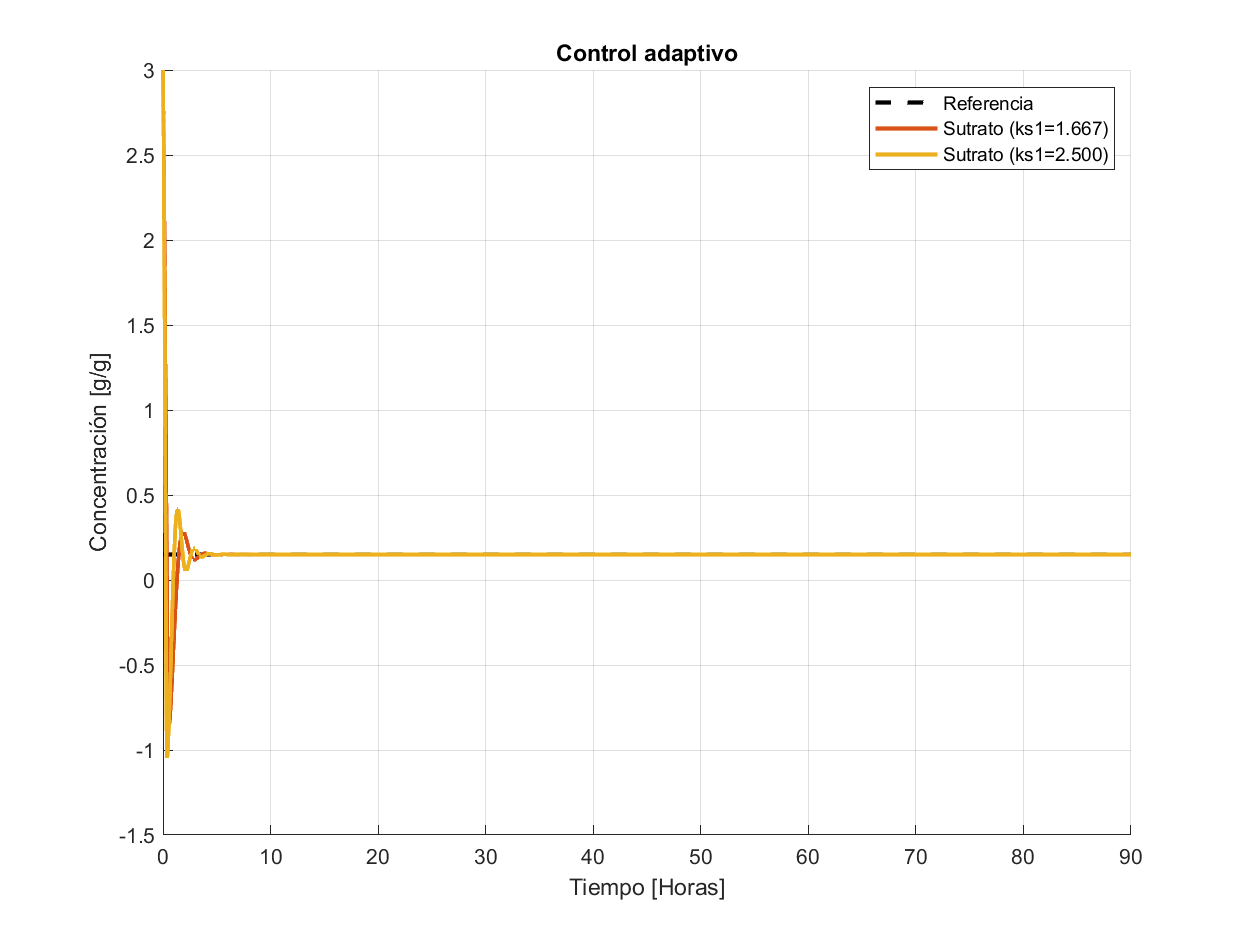
\includegraphics[width=0.43\textwidth]{./Images_tp3/ad_ks1.png}
  \caption{Control adaptivo con variaciones en $k_{s1}$}
\end{figure}
\begin{figure}[H]
  \centering
  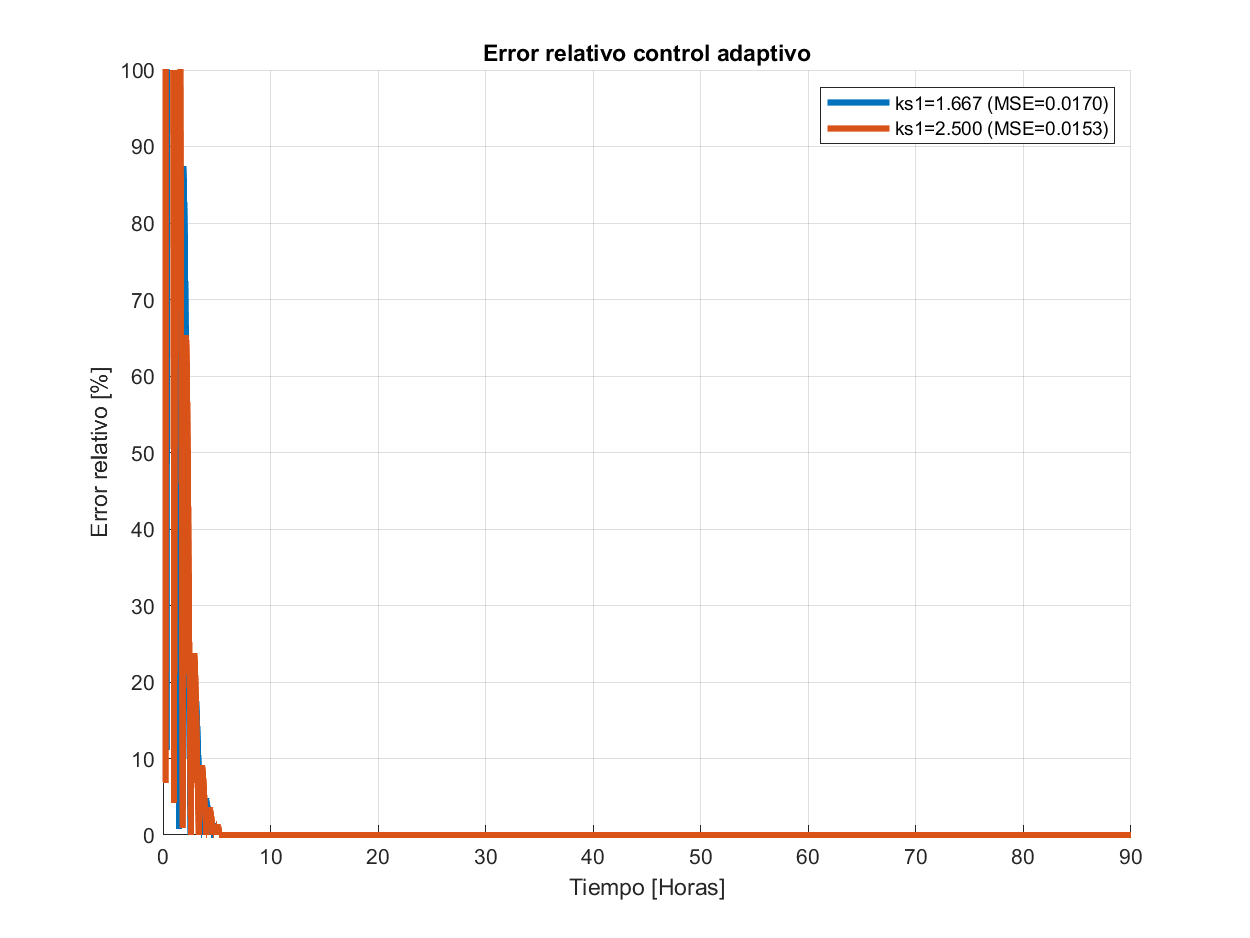
\includegraphics[width=0.43\textwidth]{./Images_tp3/ad_err_ks1.png}
  \caption{Error control adaptivo con variaciones en $k_{s1}$}
\end{figure}

\begin{figure}[H]
  \centering
  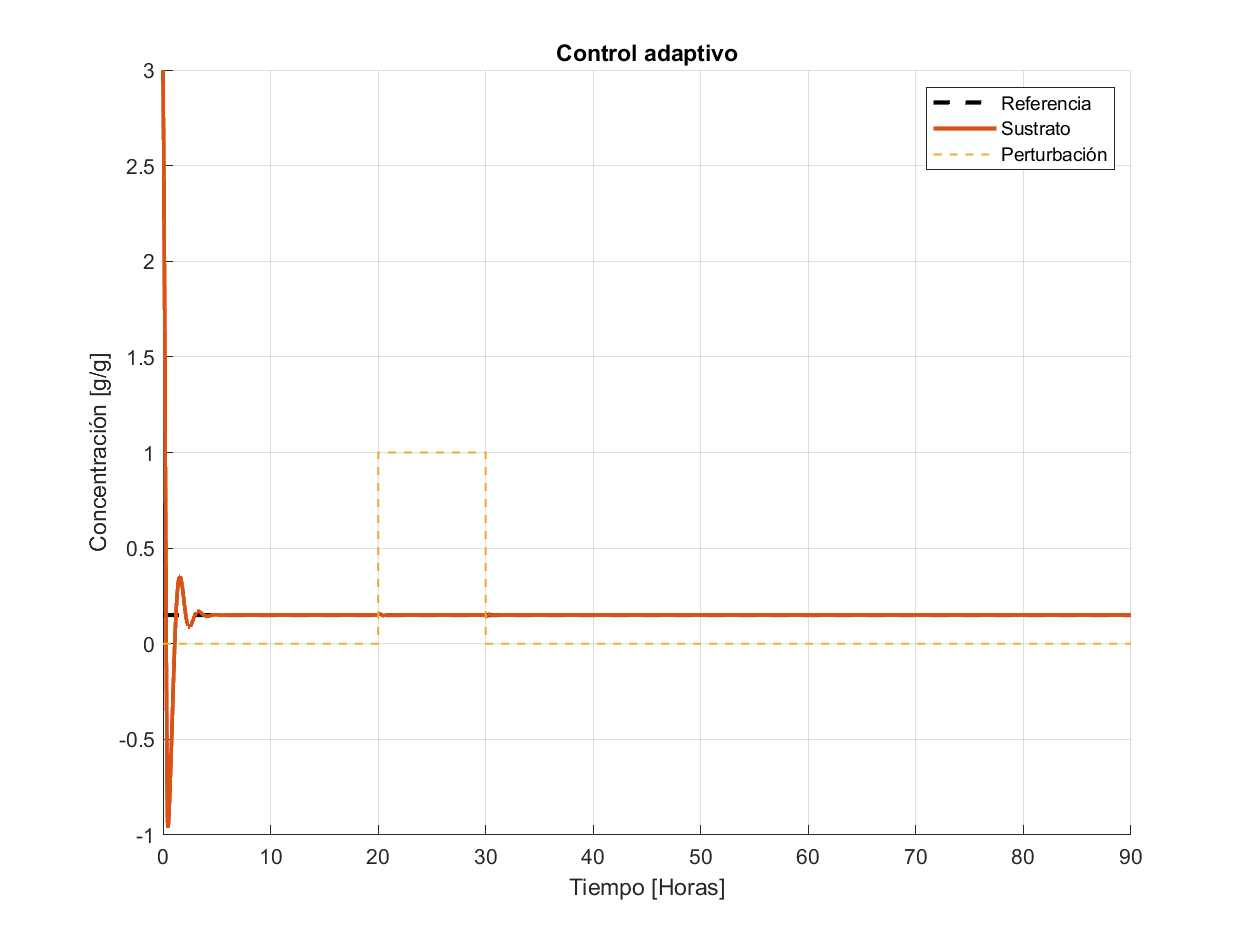
\includegraphics[width=0.43\textwidth]{./Images_tp3/ad_D.png}
  \caption{Control adaptivo con variaciones en $D$}
\end{figure}
\begin{figure}[H]
  \centering
  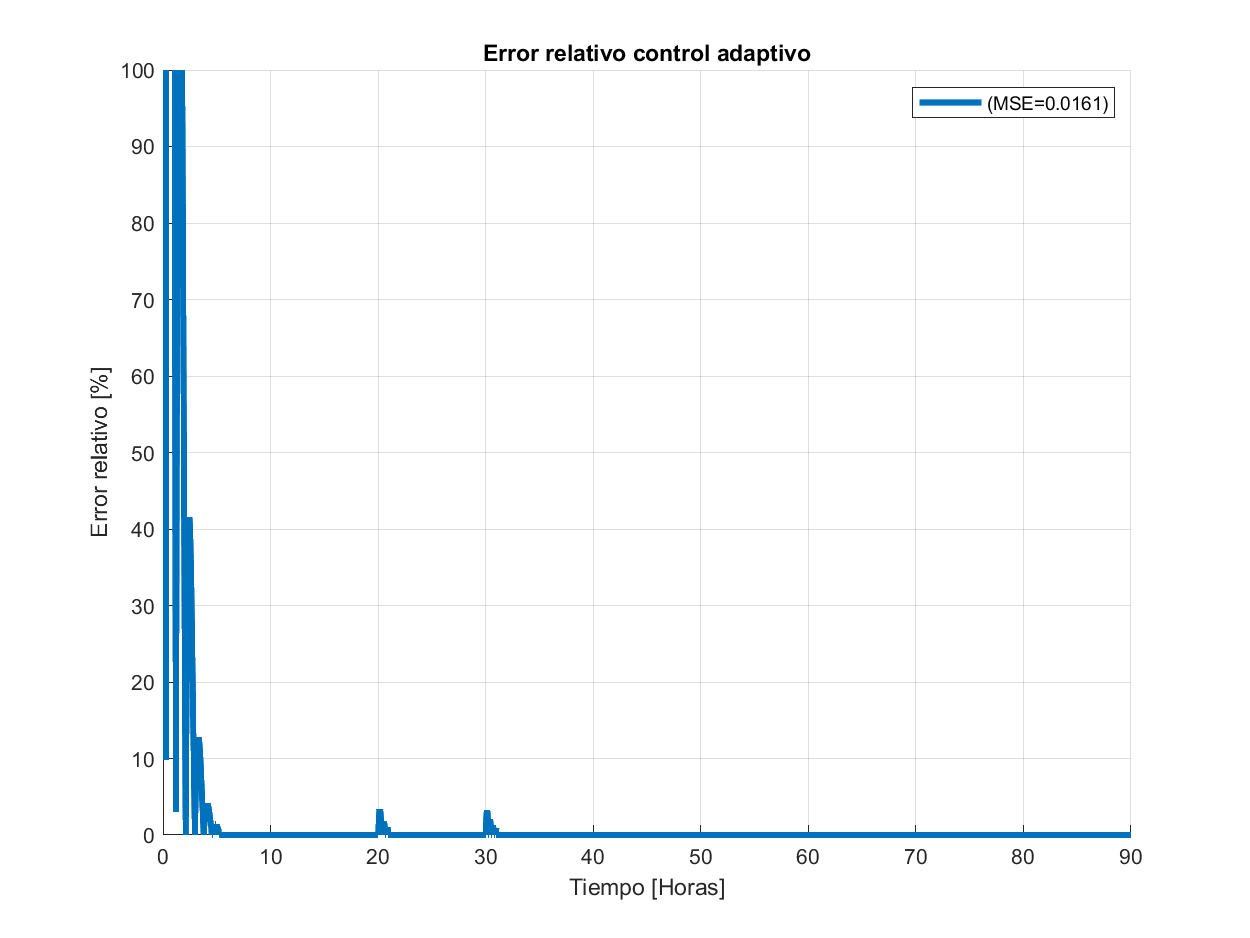
\includegraphics[width=0.43\textwidth]{./Images_tp3/ad_err_D.png}
  \caption{Error control adaptivo con variaciones en $D$}
\end{figure}

\begin{figure}[H]
  \centering
  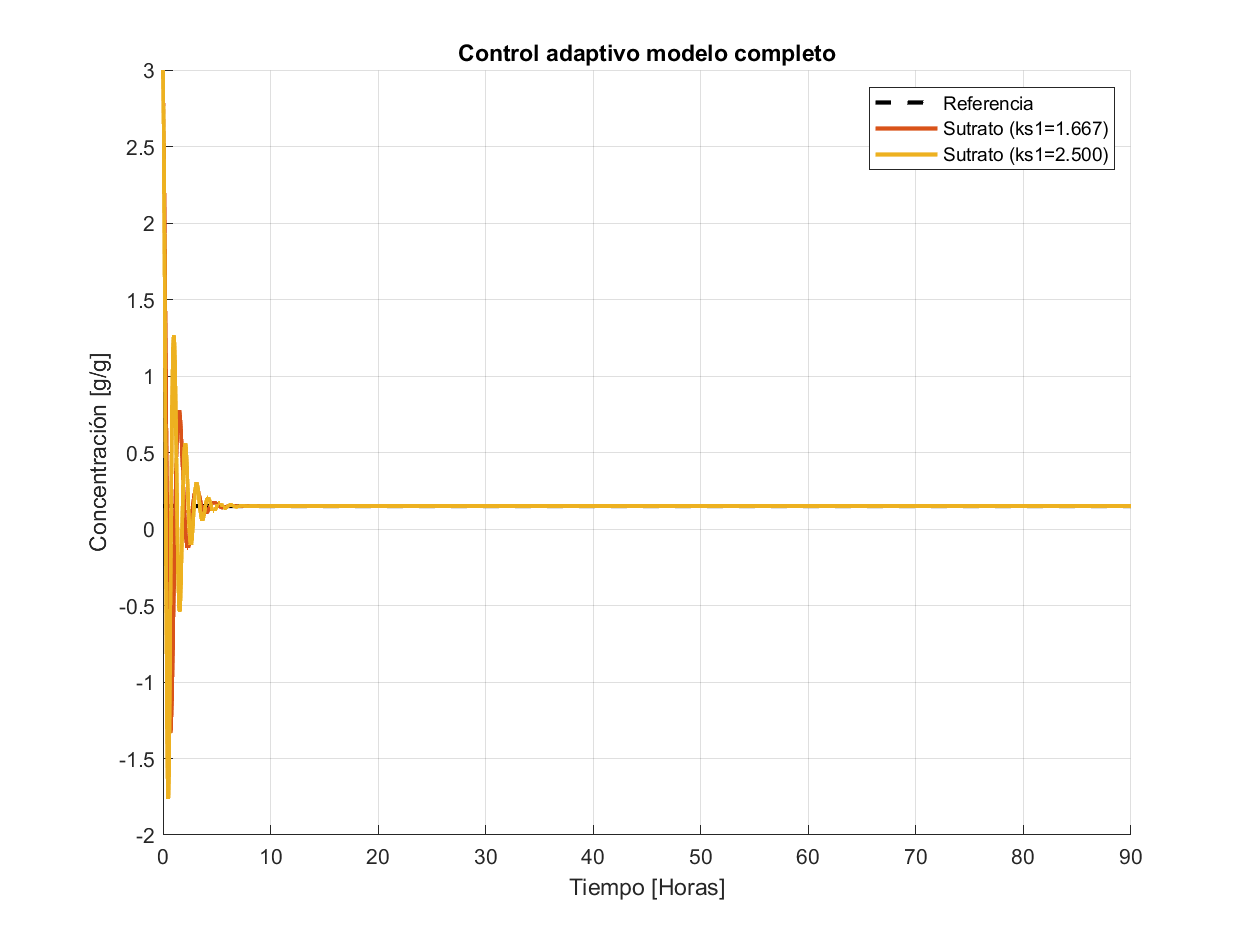
\includegraphics[width=0.43\textwidth]{./Images_tp3/ad_completo.png}
  \caption{Control adaptivo con variaciones en $k_{s1}$ modelo completo}
\end{figure}
\begin{figure}[H]
  \centering
  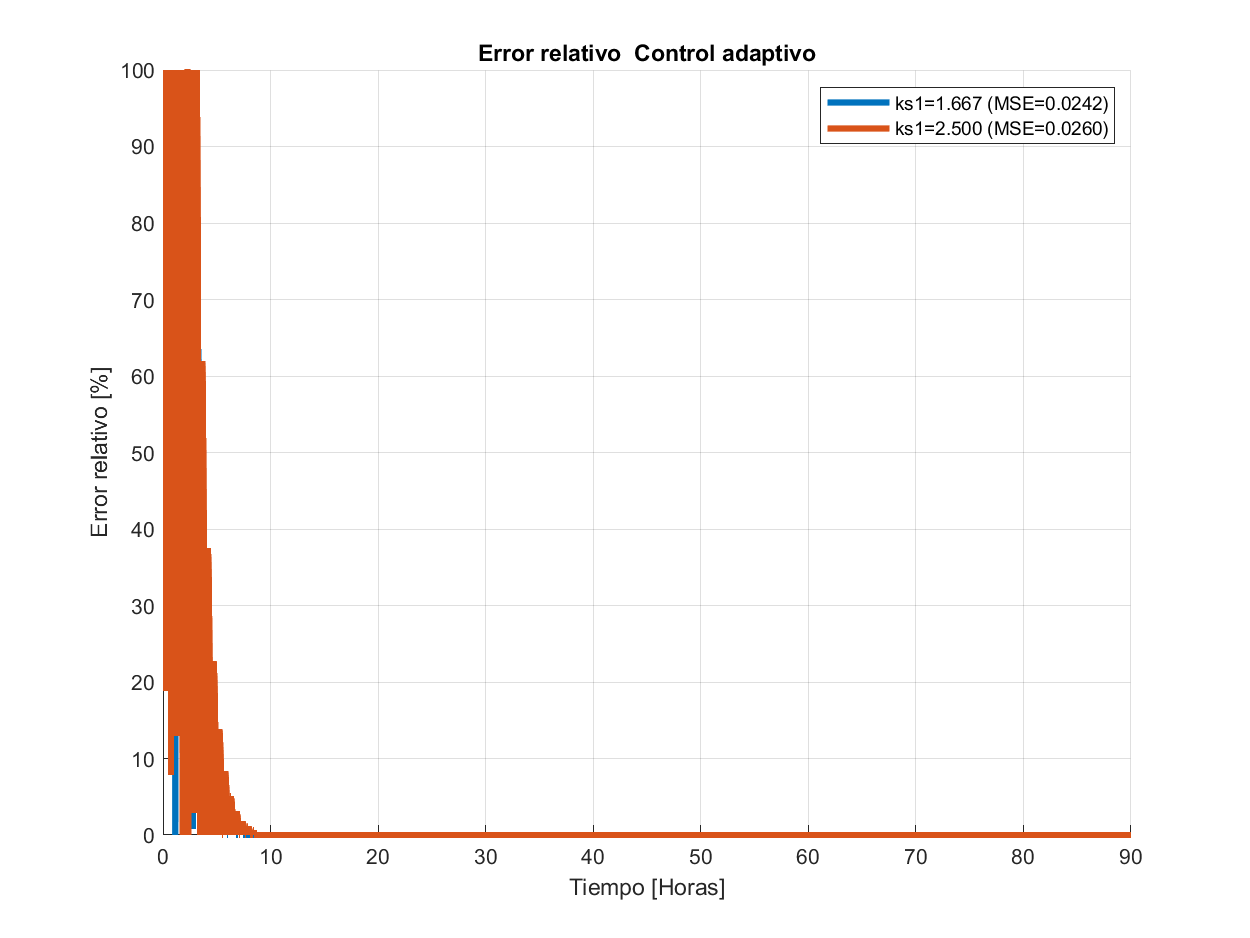
\includegraphics[width=0.43\textwidth]{./Images_tp3/ad_completo_err.png}
  \caption{Error control adaptivo con variaciones en $k_{s1}$ modelo completo}
\end{figure}

\begin{itemize}
    \item \textit{Variación de \(k_{s1}\) (\(\pm 20\%\))}: El controlador mantiene error de estado estacionario nulo y una dinámica de convergencia similar, demostrando alta robustez frente a incertidumbres en este parámetro.
    \item \textit{Variación de \(D\) (\(\pm 20\%\))}: El sistema muestra rechazo efectivo a esta perturbación, con una respuesta prácticamente invariante.
    \item \textit{Modelo completo}: Al simular con el modelo completo y variar \(k_{s1}\) en \(\pm 20\%\), se confirma que el controlador preserva su desempeño, consolidándose como una solución robusta y confiable.
\end{itemize}

\subsection{Conclusiones}
\begin{itemize}
    \item Garantiza error nulo en estado estacionario incluso ante incertidumbres en los parámetros.
    \item Ofrece un balance ajustable entre velocidad de convergencia y oscilaciones iniciales mediante \(\gamma\).
    \item Demuestra superioridad frente a los controladores tradicionales al no depender críticamente del modelo exacto del sistema.
\end{itemize}

\end{document}